%% For normal draft builds (figs undisplayed hence fast compile)
%\documentclass[hyperpdf,nobind,draft,oneside]{hepthesis}
%\documentclass[hyperpdf,nobind,draft,twoside]{hepthesis}

%% For short draft builds (breaks citations by necessity)
%\documentclass[hyperpdf,nobind,draft,hidefrontback]{hepthesis}

%%For Cambridge soft-bound version
\documentclass[bindnopdf]{heptesi}
%% For Cambridge hard-bound version (must be one-sided)
%\documentclass[hyperpdf,oneside]{hepthesis}

\newcommand{\mg}[1]{{\color{blue}{[Michele: #1]}}}

%% Load special font packages here if you wish
%\usepackage{lmodern}
\usepackage{mathpazo}
%\usepackage{euler}

%% Put package includes etc. into preamble.tex for convenience
\usepackage{xspace}
\usepackage{tikz}
\usepackage{morefloats,subfig,afterpage}
\usepackage{mathrsfs} % script font
\usepackage{verbatim}
\usepackage[hidelinks,bookmarks=true,plainpages=false]{hyperref}

%% Using Babel allows other languages to be used and mixed-in easily
%\usepackage[ngerman,english]{babel}
\usepackage[english,italian]{babel}
\selectlanguage{italian}
\usepackage[italian]{cleveref}
\usepackage{fancyvrb}

\usepackage{listings}
\lstset{
    basicstyle=\tiny\ttfamily,
    keepspaces=true,
    breaklines=true,
    postbreak=\mbox{\textcolor{red}{$\hookrightarrow$}\space},
}


\usepackage{doi}
\usepackage{url}
%\usepackage[sorting=none,maxbibnames=30,minbibnames=30]{biblatex}
\usepackage[sorting=none,minbibnames=3]{biblatex}
\addbibresource{bibliography.bib}

\newcommand\eng[1]{\foreignlanguage{english}{#1}}

%% Citation system tweaks
%\usepackage{cite}
% \let\@OldCite\cite
% \renewcommand{\cite}[1]{\mbox{\!\!\!\@OldCite{#1}}}

%% Maths
% TODO: rework or eliminate maybemath
\usepackage{abmath}
\DeclareRobustCommand{\mymath}[1]{\ensuremath{\maybebmsf{#1}}}
% \DeclareRobustCommand{\parenths}[1]{\mymath{\left({#1}\right)}\xspace}
% \DeclareRobustCommand{\braces}[1]{\mymath{\left\{{#1}\right\}}\xspace}
% \DeclareRobustCommand{\angles}[1]{\mymath{\left\langle{#1}\right\rangle}\xspace}
% \DeclareRobustCommand{\sqbracs}[1]{\mymath{\left[{#1}\right]}\xspace}
% \DeclareRobustCommand{\mods}[1]{\mymath{\left\lvert{#1}\right\rvert}\xspace}
% \DeclareRobustCommand{\modsq}[1]{\mymath{\mods{#1}^2}\xspace}
% \DeclareRobustCommand{\dblmods}[1]{\mymath{\left\lVert{#1}\right\rVert}\xspace}
% \DeclareRobustCommand{\expOf}[1]{\mymath{\exp{\!\parenths{#1}}}\xspace}
% \DeclareRobustCommand{\eexp}[1]{\mymath{e^{#1}}\xspace}
% \DeclareRobustCommand{\plusquad}{\mymath{\oplus}\xspace}
% \DeclareRobustCommand{\logOf}[1]{\mymath{\log\!\parenths{#1}}\xspace}
% \DeclareRobustCommand{\lnOf}[1]{\mymath{\ln\!\parenths{#1}}\xspace}
% \DeclareRobustCommand{\ofOrder}[1]{\mymath{\mathcal{O}\parenths{#1}}\xspace}
% \DeclareRobustCommand{\SOgroup}[1]{\mymath{\mathup{SO}\parenths{#1}}\xspace}
% \DeclareRobustCommand{\SUgroup}[1]{\mymath{\mathup{SU}\parenths{#1}}\xspace}
% \DeclareRobustCommand{\Ugroup}[1]{\mymath{\mathup{U}\parenths{#1}}\xspace}
% \DeclareRobustCommand{\I}[1]{\mymath{\mathrm{i}}\xspace}
% \DeclareRobustCommand{\colvector}[1]{\mymath{\begin{pmatrix}#1\end{pmatrix}}\xspace}
\DeclareRobustCommand{\Rate}{\mymath{\Gamma}\xspace}
\DeclareRobustCommand{\RateOf}[1]{\mymath{\Gamma}\parenths{#1}\xspace}

%% High-energy physics stuff
\usepackage{abhep}
\usepackage{hepnames}
\usepackage{hepunits}
\DeclareRobustCommand{\arXivCode}[1]{arXiv:#1}
\DeclareRobustCommand{\CP}{\ensuremath{\mathcal{CP}}\xspace}
\DeclareRobustCommand{\CPviolation}{\CP-violation\xspace}
\DeclareRobustCommand{\CPv}{\CPviolation}
\DeclareRobustCommand{\LHCb}{LHCb\xspace}
\DeclareRobustCommand{\LHC}{LHC\xspace}
\DeclareRobustCommand{\LEP}{LEP\xspace}
\DeclareRobustCommand{\CERN}{CERN\xspace}
\DeclareRobustCommand{\bphysics}{\Pbottom-physics\xspace}
\DeclareRobustCommand{\bhadron}{\Pbottom-hadron\xspace}
\DeclareRobustCommand{\Bmeson}{\PB-meson\xspace}
\DeclareRobustCommand{\bbaryon}{\Pbottom-baryon\xspace}
\DeclareRobustCommand{\Bdecay}{\PB-decay\xspace}
\DeclareRobustCommand{\bdecay}{\Pbottom-decay\xspace}
\DeclareRobustCommand{\BToKPi}{\HepProcess{ \PB \to \PK \Ppi }\xspace}
\DeclareRobustCommand{\BToPiPi}{\HepProcess{ \PB \to \Ppi \Ppi }\xspace}
\DeclareRobustCommand{\BToKK}{\HepProcess{ \PB \to \PK \PK }\xspace}
\DeclareRobustCommand{\BToRhoPi}{\HepProcess{ \PB \to \Prho \Ppi }\xspace}
\DeclareRobustCommand{\BToRhoRho}{\HepProcess{ \PB \to \Prho \Prho }\xspace}
\DeclareRobustCommand{\X}{\thesismath{X}\xspace}
\DeclareRobustCommand{\Xbar}{\thesismath{\overline{X}}\xspace}
\DeclareRobustCommand{\Xzero}{\HepGenParticle{X}{}{0}\xspace}
\DeclareRobustCommand{\Xzerobar}{\HepGenAntiParticle{X}{}{0}\xspace}
\DeclareRobustCommand{\epluseminus}{\Ppositron\!\Pelectron\xspace}
\DeclareRobustCommand{\protonproton}{\Pproton\APantiproton\xspace}


%% You can set the line spacing this way
%\setallspacing{double}
%% or a section at a time like this
%\setfrontmatterspacing{double}


%% Define the thesis title and author
% \title{}
% \author{}

%% Qua c'è una guida di hepthesis (https://ctan.org/pkg/hepthesis)
%% https://ctan.mirror.garr.it/mirrors/ctan/macros/latex/contrib/hepthesis/hepthesis.pdf

%% Doc-specific PDF metadata
\makeatletter
\@ifpackageloaded{hyperref}{%
\hypersetup{%
  pdftitle = {Virtualizzazione di Funzioni di Rete},
  pdfsubject = {Network Functions Virtualization},
  pdfkeywords = {NFV, SDN, KVM, DPDK, VPP},
  pdfauthor = {\textcopyright\ Samuele Pilleri}
}}{}
\makeatother


%% Start the document
\begin{document}

%% Define the un-numbered front matter (cover pages, rubrik and table of contents)
\begin{frontmatter}
  \begin{titlepage}

\vspace{-12em}

\begin{addmargin}[.3cm]{.3cm}
\begin{center}

\large

{\textsc UNIVERSIT\`A DEGLI STUDI DI TORINO}

{\textsc DIPARTIMENTO DI INFORMATICA}

{\textsc SCUOLA DI SCIENZE DELLA NATURA}

{\textsc Corso di Laurea Magistrale in Informatica}


\vskip 30 pt

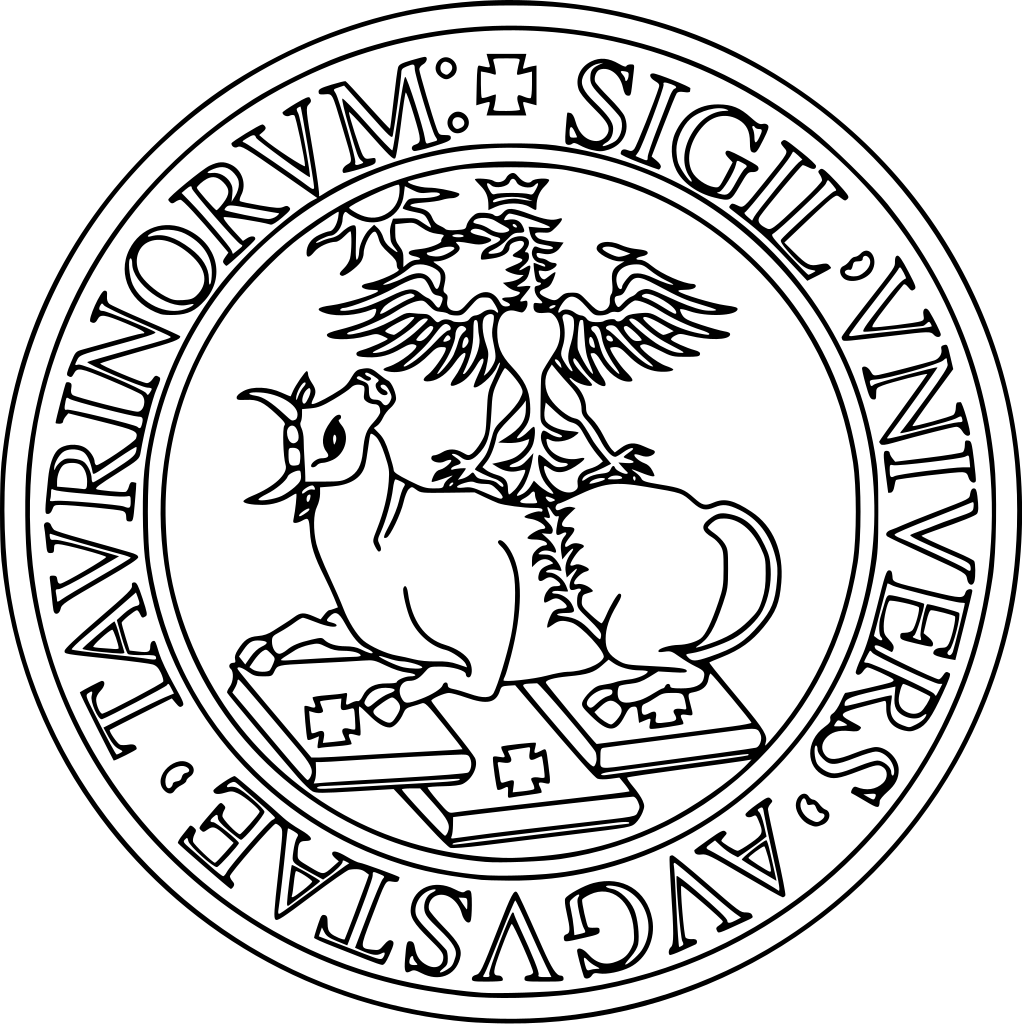
\includegraphics[width=6cm]{graphics/logo.png}

\vskip 30pt

\normalsize {Tesi di Laurea Magistrale}

\vskip 30pt

\Huge\textbf{Virtualizzazione di Funzioni di Rete}

\large

\vskip 30pt

\noindent \textbf{Relatore:} Prof. Michele Garetto
\hfill \textbf{Candidato:}
\\
\noindent \textbf{Correlatore:} Ing. Alessandro Galardini
\hfill Samuele Pilleri

\vskip 30pt


A.A. 2020/2021 \\
Sessione di Giugno 2022

\end{center}
\end{addmargin}

\end{titlepage}
  
  \thispagestyle{empty}

%% Abstract
\begin{abstract}%[\smaller \thetitle\\ \vspace*{1cm} \smaller {\theauthor}]
  %\thispagestyle{empty}
  Nell'ultimo decennio il settore delle telecomunicazioni ha visto la nascita di molteplici iniziative con il comune obiettivo di creare un ecosistema hardware e software aperto per le reti Internet, superando il modello chiuso proposto dai Vendor tradizionali. In questo scenario, il software riveste un ruolo chiave: dal 5G all'edge computing, le nuove architetture devono essere flessibili, scalabili ed economiche. Si inizia quindi a parlare di \textit{telco cloud}, dove le prestazioni e il \mbox{management} evoluto delle odierne piattaforme di virtualizzazione, basate su hypervisor e container, permettono di implementare in maniera efficace e flessibile le funzioni di rete prima vincolate al deploy di appliance fisiche.

  Lo scopo di questa tesi è in primis fornire una panoramica sullo stack tecnologico hardware e software necessario per realizzare l'architettura, descrivendone lo stato dell'arte, le varie componenti in gioco e come si integrano tra loro. In secondo luogo, si propone un'architettura virtuale che realizzi una particolare funzione, il \mbox{peering} decentralizzato all'edge della rete, studiandone le performance attraverso i principali indicatori.
\end{abstract}


%% Declaration
\begin{declaration}
  Dichiaro di essere responsabile del contenuto dell'elaborato che presento al fine del
  conseguimento del titolo, di non avere plagiato in tutto o in parte il lavoro prodotto da
  altri e di aver citato le fonti originali in modo congruente alle normative vigenti in
  materia di plagio e di diritto d'autore. Sono inoltre consapevole che nel caso la mia
  dichiarazione risultasse mendace, potrei incorrere nelle sanzioni previste dalla legge e la
  mia ammissione alla prova finale potrebbe essere negata.
  \vspace*{1cm}
  \begin{flushright}
    Samuele Pilleri
  \end{flushright}
\end{declaration}


% % Acknowledgements
% \begin{acknowledgements}
%   Ringrazio i miei familiari ed i loro sforzi che mi hanno permesso, pur non senza intoppi, di raggiungere questa tanto agognata meta.
  
%   Ringrazio i professori, presenti e passati, le cui lezioni continueranno ad arricchirmi anche dopo la fine della scuola.
  
%   Ringrazio i miei amici, anche quelli del baretto, per avermi ispirato, incoraggiato, sopportato e per i momenti di leggerezza vissuti insieme.
  
%   Ma il grazie più sentito va al mio mentore, Alessandro, conosciuto per caso in un gruppo Telegram: a te sono grato di avermi spalancato le porte delle telco, accogliendomi nel piccolo giardino del TOP-IX e facendomi sentire subito a casa. Mi hai guidato nel muovere i primi passi verso il raggiante futuro che ci aspetta, senza mai essere avaro di sapere. Quelli trascorsi in via delle Rosine sono stati i sei mesi più ricchi da quando mi sono immatricolato, non lo dimenticherò mai.
  
%   Grazie a tutti voi questo lavoro è stato svolto non solo con passione, ma con gioia!
% \end{acknowledgements}


%% Preface
% \begin{preface}
%   This thesis describes my research on various aspects of the \LHCb
%   particle physics program, centred around the \LHCb detector and \LHC
%   accelerator at \CERN in Geneva.

%   \noindent
%   For this example, I'll just mention \ChapterRef{chap:SomeStuff}
%   and \ChapterRef{chap:MoreStuff}.
% \end{preface}

%% ToC
\tableofcontents


%% Strictly optional!
\frontquote{%
  Non chi comincia, ma quel che persevera.}%
  {Leonardo da Vinci}
%% I don't want a page number on the following blank page either.
\thispagestyle{empty}

\end{frontmatter}

%% Start the content body of the thesis
\begin{mainmatter}
  \chapter{Introduzione}
\label{chap:intro}

%% Restart the numbering to make sure that this is definitely page #1!
\pagenumbering{arabic}

La concezione di Internet come la conosciamo oggi esiste dagli anni settanta, ma il modo di realizzarla è ampiamente mutato nel tempo, adattandosi alle tecnologie disponibili nelle varie epoche, e sempre con un occhio di riguardo alla resilienza.

L'approccio tradizionale è fortemente incentrato sui \textit{Vendor}, ossia i fornitori di soluzioni chiavi in mano che curano ogni aspetto della progettazione degli apparati, hardware e software, offrendo prodotti testati e completi sotto il profilo funzionale, al punto che l'unico compito del tecnico di rete è quello di configurarli prima che possano essere operativi. Ciò ha sicuramente dei vantaggi poiché consente di creare un ecosistema coeso e compatto, in cui tutte le risorse sono sfruttate al massimo delle loro potenzialità, e la compatibilità delle diverse componenti è garantita dal produttore. Il rovescio della medaglia è l'esacerbazione di tutte quelle politiche di mercato monopolistiche che mirano a chiudere gli acquirenti in una cosiddetta ``gabbia dorata'' al fine di vendere loro supporto tecnico a pagamento e altri prodotti affini e complementari, sfavorendo l'integrazione con soluzioni concorrenti nonostante i protocolli principali siano stati resi interoperabili pubblicando standard RFC aperti.

Il problema è molto sentito, tanto che negli anni hanno preso vita due diversi filoni di ricerca con lo scopo di arginare lo strapotere dei produttori. Il primo, noto come \textit{Software Defined Networking}, mira ad astrarre ed in qualche modo unificare la configurazione della rete, in maniera che possa essere controllata da un software centralizzato superando la necessità di intervenire su ciascun apparato singolarmente. Il secondo invece riguarda gli algoritmi, la logica e le funzioni degli apparati ed è l'argomento di questa tesi.

\section{Data plane e Control plane}

Occorre innanzitutto effettuare una distinzione in termini ed inquadrare due concetti centrali attorno ai quali ruotano buona parte degli argomenti che hanno da sempre caratterizzato il mondo del networking.

Si pensi ad una strada trafficata. Le protagoniste sono ovviamente le automobili, semplici e veloci, che vogliono recarsi da un punto A ad un punto B nel più breve tempo possibile. Per riuscirvi però hanno bisogno di coordinarsi tra loro ed orientarsi per trovare la strada migliore lungo il percorso. Ecco quindi che subentrano semafori, segnaletica ed indicazioni che hanno la funzione di regolare il traffico, guidarlo e spostarlo in caso di incidenti, code o altri avvenimenti avversi.

In Internet lo scenario è analogo: i pacchetti dati, rappresentati dalle auto, devono raggiungere rapidamente la destinazione prefissata scorrendo attraverso i nodi della rete, il \textit{data plane} (o \textit{forwarding plane}), e per farcela hanno bisogno di un sistema che indichi loro la direzione. Il compito ricade sul \textit{control plane} che, interagendo con gli altri nodi, ricostruisce una visione globale della rete e determina le migliori direzioni da intraprendere per raggiungere la meta. L'output del control plane costituisce quindi un tassello fondamentale del data plane, ed il reciproco disaccoppiamento permette ai due di evolversi parallelamente. È il caso di diversi algoritmi di routing, come OSPF, IS-IS e BGP, operanti sul control plane e aventi come obiettivo quello di produrre le tabelle di forwarding necessarie al data plane.

In generale, si considera piano di inoltro quell'insieme di operazioni che avvengono ai livelli 2 e 3 dello stack ISO/OSI, mentre il control plane è realizzato da protocolli applicativi di livello 7. Il confine ad ogni modo non è netto, tanto che soluzioni come il NAT, operante ai livelli 3 e 4, sono considerate parte del data plane.

\section{SDN e NFV}
\label{sec:sdn-nfv}

La separazione ideale trova riscontro nell'architettura, nell'hardware e nei protocolli che implementano la rete. Nei router commerciali tradizionali è comune trovare dei circuiti integrati dedicati a gestire efficacemente il forwarding sul data plane (i cosiddetti \textit{ASIC}) a fianco di processori general purpose che hanno il compito di farsi carico del sistema operativo del router e del suo control plane. Queste scelte progettuali hanno avuto il merito di guidare lo sviluppo di Internet, determinando l'evoluzione dei protocolli necessari per gestire architetture sempre più articolate. In questa concezione ogni apparato, sia esso un router, uno switch o di altra natura, è a sé stante e comunica costantemente coi suoi vicini. Si è dunque dinanzi ad un algoritmo distribuito, in cui ciascun oggetto è un'istanza di una particolare funzione che interagisce con le altre scambiandosi messaggi grazie ai quali effettuare scelte locali che avranno ripercussione sull'intera rete.

\begin{figure}[htb]
    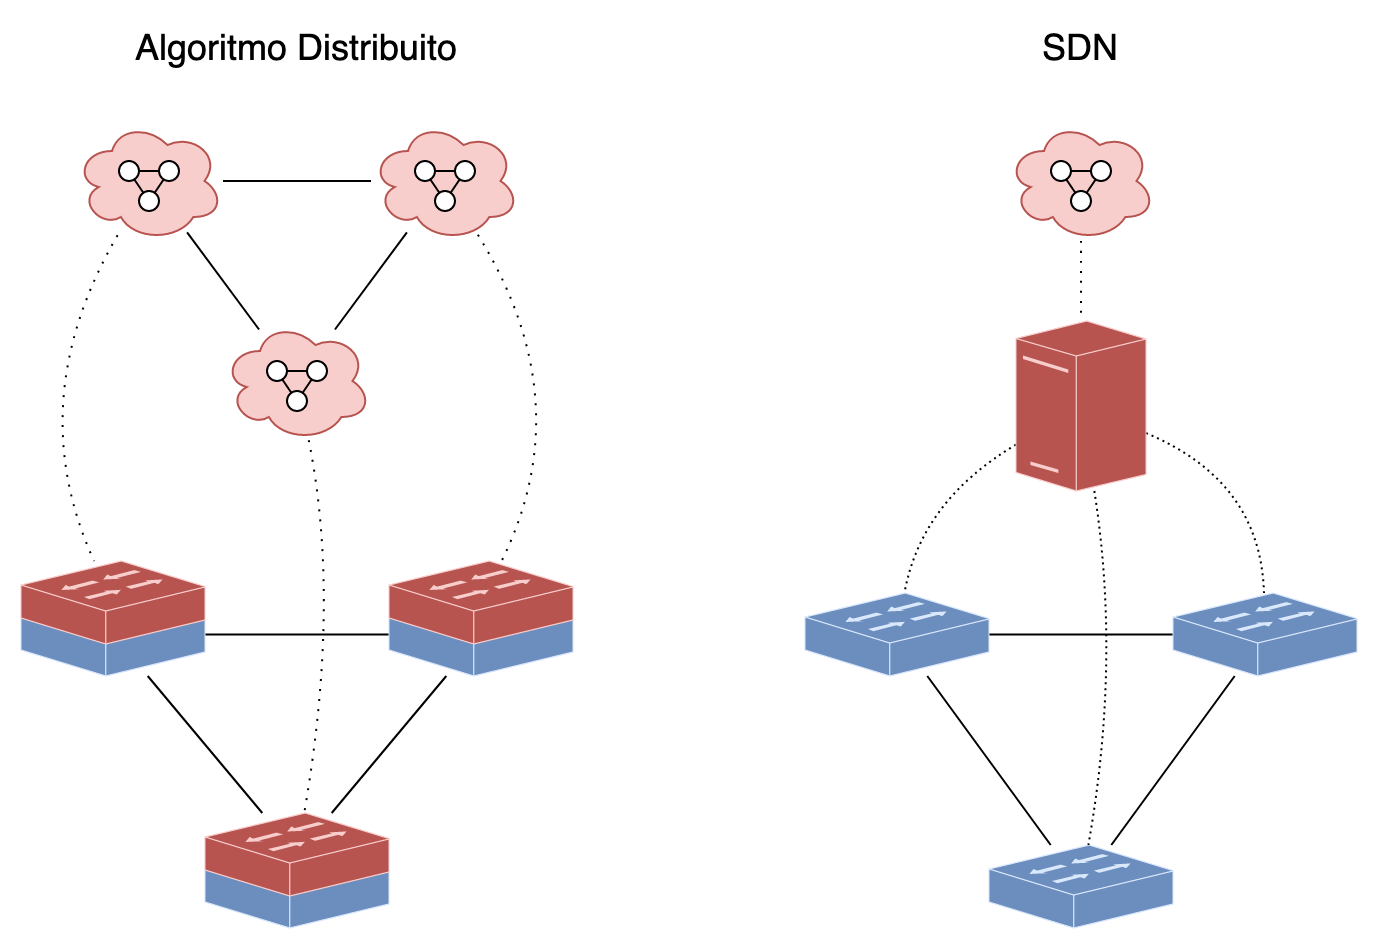
\includegraphics[width=0.7\textwidth]{graphics/trad-vs-sdn.png}
    \caption{Differenza tra approccio tradizionale e SDN}
    \label{fig:trad-vs-sdn}
\end{figure}

Questo approccio, seppur molto valido da un punto di vista teorico, ha dei limiti legati alla difficoltà di realizzare funzioni di complessità crescente e all'impossibilità di convergere rapidamente in caso di guasti. Inoltre è incentrato su valutazioni di tipo topologico e non tiene conto delle condizioni di rete come il livello di congestione di un collegamento che può impattare sull'esperienza d'uso da parte degli utenti, né considera le dinamiche economiche legate alla gestione e alla diversificazione del traffico.

Nell'ultimo decennio, grazie al graduale abbattimento dei costi dell'hardware ed allo sviluppo di soluzioni software sempre più sofisticate, ha preso forma un nuovo modo di costruire le reti, in cui il disaccoppiamento tra data plane e control plane non è più solo logico, ma anche fisico. Si tratta del \textit{Software Defined Networking} (SDN) in cui il data plane è affidato a delle appliance fisiche genericamente chiamate ``switch'' dislocate nei vari nodi, mentre il control plane è centralizzato su server ridondati noti come ``controller'' (\cref{fig:trad-vs-sdn}). La prima soluzione di successo largamente adottata di questo paradigma è OpenFlow, un protocollo aperto che implementa la cosiddetta ``Southbound API'', ossia l'interfaccia di comunicazione tra controllori e switch.

Se da un lato SDN rilassa il legame tra piano dati e di controllo, rimane ancora aperto l'interrogativo su come debba essere realizzato quest'ultimo. Per rispondere a questa domanda, occorre prima individuare i compiti che esso svolge. Oltre a gestire gli algoritmi di instradamento, il control plane si occupa anche di autenticazione ed accounting delle sessioni utente, interconnessione con altre reti, allocazione di risorse per determinati servizi ed in generale tutte quelle forme di governance da cui dipende il transito dei dati sulla rete. A questa dimensione, va aggiunta anche quella delle funzioni della rete e dei servizi che essa offre. Ad esempio si parla di caching dei contenuti tramite le Content Delivery Network (CDN), firewalling, NAT, più tutte le funzioni intermedie necessarie a realizzare architetture più complesse, come quelle proprie della telefonia mobile.

Da questi interrogativi è partita la cordata di 13 grandi operatori Internet che nel 2012 ha dato impulso alla nascita di un segmento di ricerca chiamato \textit{Network Functions Virtualization} (NFV), o virtualizzazione di funzioni di rete \cite{nfvwhitepaper1}. Gli obiettivi erano chiari: superare il modello chiuso imposto dai vendor e realizzare un ecosistema aperto in cui il software del piano di controllo e le relative funzioni potessero risiedere fuori dalle appliance dedicate. Tecnologie di virtualizzazione emergenti come macchine virtuali e container potevano essere sfruttate per ospitare le funzioni su server comuni, meglio conosciuti col nome Commercial Off-The-Shelf (COTS). Un'altra opportunità era rappresentata dai dispositivi ``white box'', router e switch molto veloci risultato del matrimonio tra due realtà: le grandi aziende del silicio, in grado di progettare chip dedicati al data plane, e i produttori di soluzioni integrate. Questa famiglia di device in particolare è sempre più numerosa poiché permette di coniugare prestazioni e flessibilità. Tra i primi ad intraprendere questo percorso vi fu Nvidia che realizzò switch SDN mossi da ASIC Mellanox (poi acquisita) e animati da Cumulus Linux, una distribuzione realizzata ad hoc in grado di mettere a fattor comune merchant silicon con un control plane containerizzato.

\begin{figure}[htb]
    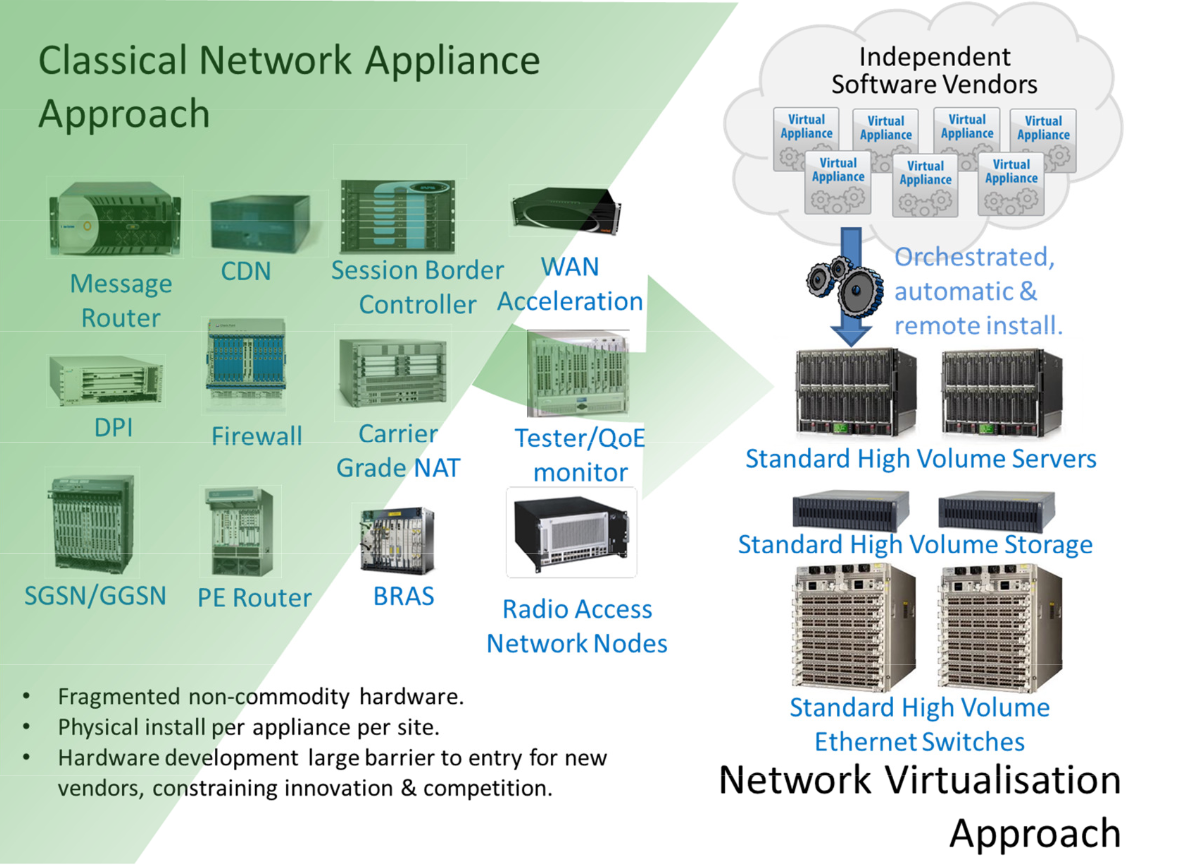
\includegraphics[width=0.7\textwidth]{graphics/trad-vs-nfv.png}
    \caption{Verso NFV}
    \label{fig:trad-vs-nfv}
\end{figure}

Dividere le responsabilità consente di razionalizzare i costi degli apparati fisici, ottimizzare gli investimenti e favorire l'integrazione di soluzioni diverse grazie al contributo dell'open source. L'architettura proposta verrà meglio trattata nel prossimo paragrafo, tuttavia è bene anticipare che le due filosofie, classica e moderna, possono coesistere: ad esempio si può adottare lo stack moderno all'interno dei data center lasciando algoritmi ed apparati tradizionali a gestire le comunicazioni su scala geografica. La divisione tra piano dati e di controllo offre infatti ampi spazi di manovra e lascia al progettista la libertà di implementare l'innovazione senza compromettere quanto di già funzionante esiste nella rete.

\section{ETSI NFV}

L'incipit dei 13 fu raccolto da ETSI, lo European Telecommunications Standards Institute, che creò un Industry Specification Group (ISG) dedicato a NFV con lo scopo di coordinare gli sforzi dei vari operatori: nel giro di pochi anni, infatti, oltre un centinaio di aziende ed enti si dimostrarono interessati all'argomento.

Durante il processo di definizione dei requisiti, ETSI preparò un framework architetturale di riferimento il cui scopo era focalizzarsi sui blocchi funzionali e sui punti di riferimento che sarebbero emersi dalla progettazione della nuova architettura \cite{estinfv002}.

\begin{figure}[htb]
    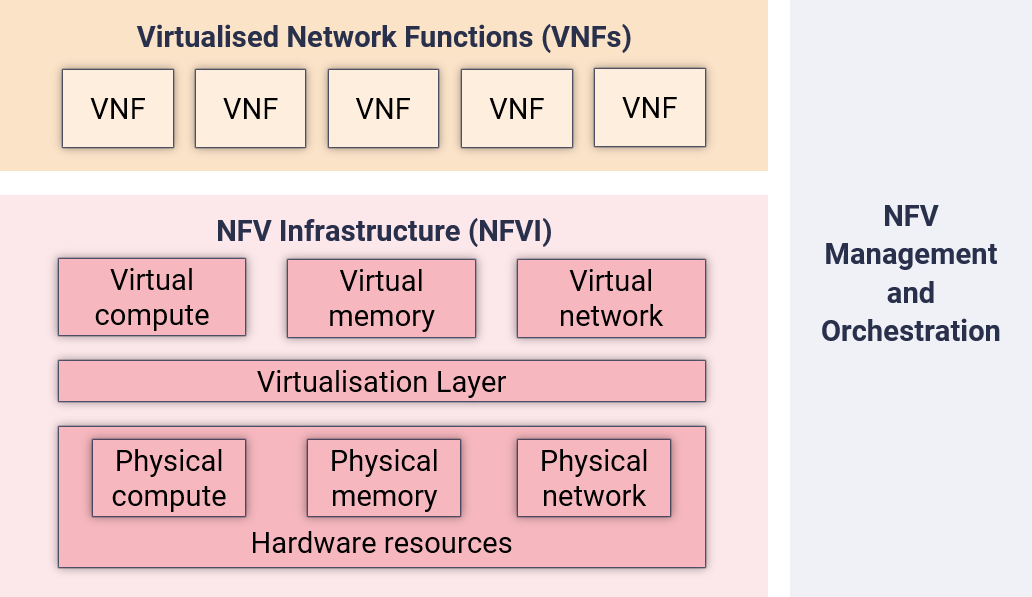
\includegraphics[width=0.7\textwidth]{graphics/high-level_etsi_framework.png}
    \caption{Schema ad alto livello del framework ETSI NFV}
    \label{fig:esti-nfv-high-level}
\end{figure}

Da una visione ad alto livello del lavoro prodotto dal gruppo, si distinguono tre componenti principali (\cref{fig:esti-nfv-high-level}):

\begin{enumerate}
    \item Le Virtualized Network Functions (VNFs), ossia le vere e proprie funzioni del control plane che s'intende virtualizzare. È logico aspettarsi che ognuna di esse sia contraddistinta da dei requisiti, come la necessità di hardware specifico per poter funzionare, ed altre informazioni a corredo.
    \item La NFV Infrastructure (NFVI), cioè le componenti fisiche su cui eseguire le funzioni. Per garantire la flessibilità dell'architettura, le risorse fisiche vengono astratte e presentate alle VNFs sotto forma di risorse virtuali.
    \item NFV Management and Orchestration (MANO), componente trasversale che ha funzioni di controllo sull'architettura, come il monitoring, l'assegnazione delle risorse infrastrutturali alle VNFs e la gestione del loro ciclo di vita.
\end{enumerate}

È importante notare come ciascuno di questi tre blocchi non sia un prodotto finito, ma piuttosto una specifica ad alto livello dei compiti ricoperti dal corrispettivo attore. Non si parla quindi di macchine virtuali o container per le funzioni virtuali, così come non si fa riferimento ad alcun specifico virtualizzatore per l'astrazione delle risorse. Lo stesso vale per la componente di Management and Orchestration di cui però viene fornita un'implementazione di riferimento sotto il nome di \textit{Open Source MANO}.

\begin{figure}[htb]
    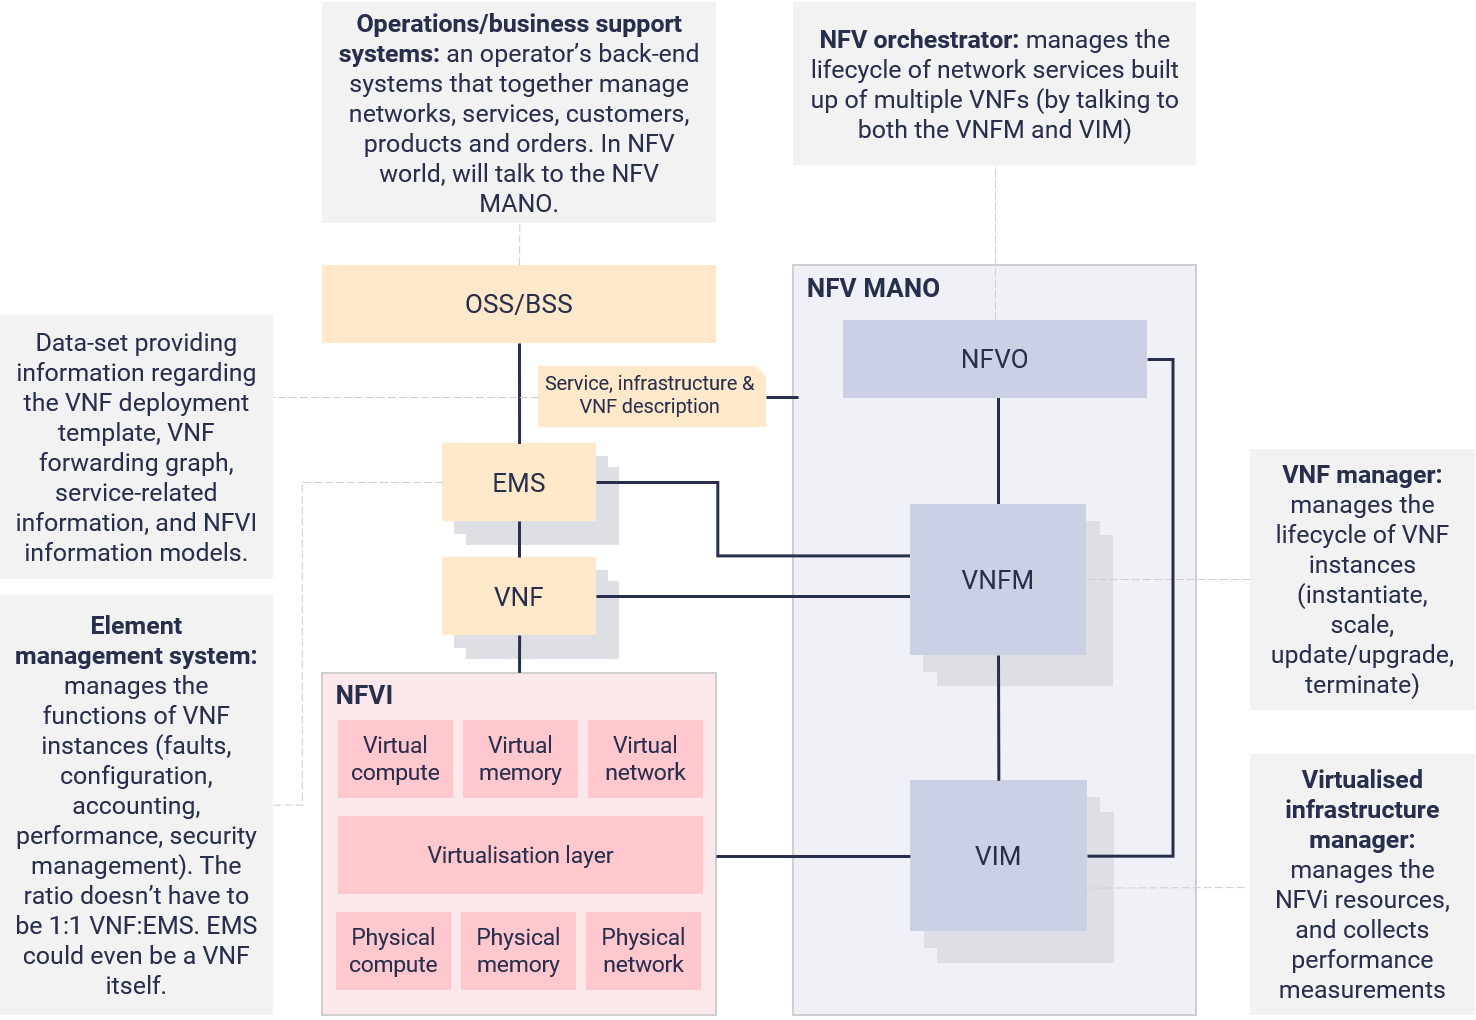
\includegraphics[width=0.7\textwidth]{graphics/full_etsi_framework.png}
    \caption{Schema dettagliato del framework ETSI NFV}
    \label{fig:esti-nfv-low-level}
\end{figure}

La natura agnostica dell'architettura proposta emerge ancor più chiaramente dallo schema dettagliato di ETSI (\cref{fig:esti-nfv-low-level}) dove ciascun blocco funzionale viene spiegato alla luce delle sotto-unità di cui è composto e di come queste comunichino tra loro.

\section{Obiettivi}

L'incipit di questa tesi nasce da un articolo in cui un grande operatore nazionale descrive la nuova architettura della propria rete geografica \cite{revolutiontim}. Questa, come da prassi consolidata, è fisicamente organizzata in anelli simili ad un fiore: al centro si trova la rete core, il pistillo attorno al quale si sviluppano le corone di petali, ossia le reti di trasporto, raccolta e accesso. I vantaggi principali della struttura ad anelli consistono nell'omogeneità progettuale e nell'innata resilienza: da ogni nodo esistono due percorsi per raggiungere lo strato superiore, potendo assicurare un ripiego immediato in caso di guasti.

Dal punto di vista logico ogni livello è caratterizzato da tecnologie diverse. La struttura gerarchica della rete, che concentra il traffico verso il cuore, determina un differenziale nella capacità trasmissiva necessaria, che è minore verso le sedi periferiche e via via crescente verso il livello intermedio di aggregazione e poi verso gli stessi nodi core. Storicamente gli elementi di rete più periferici erano anche i meno sofisticati, fattore che ha contribuito a ridurre i costi data la loro abbondanza. Il risultato è che le reti di accesso e raccolta erano gestite come domini di livello 2 e la ridondanza ottenuta tramite protocolli di spanning tree.

\begin{figure}[htb]
    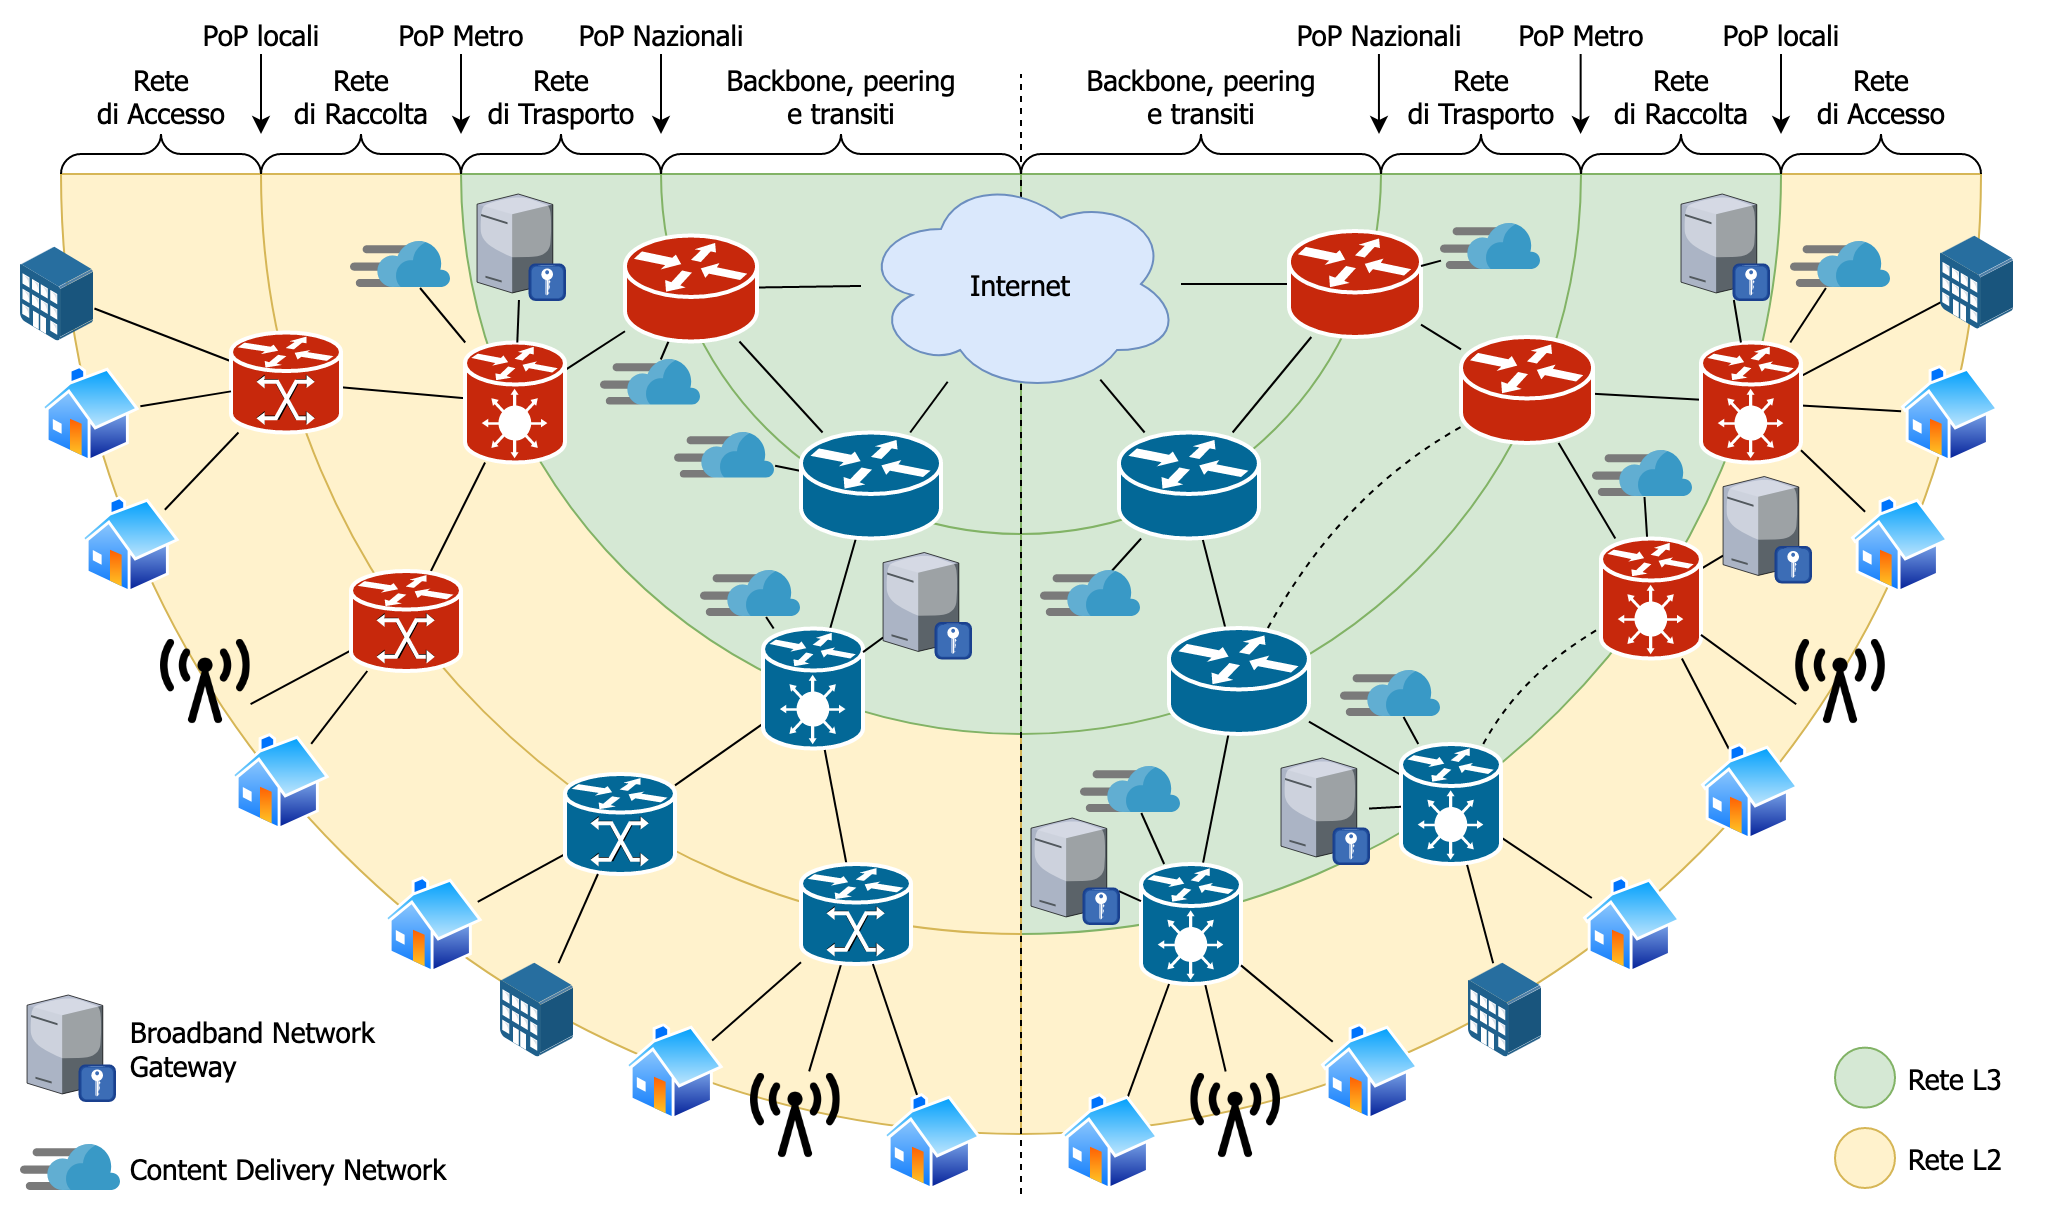
\includegraphics[width=0.8\textwidth]{graphics/isp-arch.png}
    \caption{Le due architetture a confronto}
    \label{fig:isp-arch}
    \begin{adjustwidth}{0.1\textwidth}{0.1\textwidth}
        \centering
        \footnotesize A sinistra lo schema di due reti di accesso e raccolta interamente switchate, a destra un modello con IP fino ai PoP locali. Si noti come nella nuova architettura sia possibile interconnettersi ed erogare servizi all'edge.
    \end{adjustwidth}
\end{figure}

Di recente l'aumento dell'uso di Internet ha definito la necessità di offrire servizi geograficamente vicini agli utenti che altrimenti avrebbero saturato le dorsali per usufruirne: dallo smart working allo streaming sportivo, passando per i contenuti on demand e la rete mobile, la mole di traffico aumenta più velocemente di quanto non progredisca la tecnologia e l'unico modo di stare al passo è distribuire il carico in più punti accorciando altresì la distanza tra domanda e offerta. S'inizia dunque a parlare di \textit{edge computing}, contrapposto alla visione centralizzata. CDN, centralini VoIP e perfino elementi della rete 5G devono trovare posto ai bordi. Per riuscirvi però è necessario rivedere la rete, introducendo il livello IP laddove prima non era presente.

Riprogettare offre l'opportunità unica di sbizzarrirsi e sperimentare nuove idee, partendo da una tela bianca. Perché dunque non immaginare un'architettura completamente virtuale, orchestrata su moderni sistemi software, in cui ogni funzione, ivi compreso il routing, è realizzata su server ad alte prestazioni? A questo punto persino il \textit{peering decentralizzato all'edge su architettura cloud} diventa una prospettiva conquistabile. Nei prossimi capitoli descriverò il nostro tentativo, focalizzando la narrativa sulle tecnologie, sui sistemi, sulle difficoltà riscontrate e sui risultati.
  \chapter{Software}
\label{chap:software}

Proprio come nel libro di James Kurose e Keith Ross, quest'analisi inizia dall'alto. Il tema della tesi è infatti intrinsecamente duplice: da un lato si parla delle funzioni di rete, ossia del software oggi confinato in soluzioni proprietarie, e di come queste si stiano pian piano aprendo un varco nel mondo open source, anche grazie al contributo inaspettato degli storici padroni del mercato. La seconda parte invece riguarda le tecnologie necessarie a realizzare l'infrastruttura virtuale e troverà spazio nel \cref{chap:virt}.

\section{DPDK}
\label{sec:dpdk}

Il fulcro di questa piccola rivoluzione è il \textit{Data Plane Development Kit} (DPDK), una libreria software aperta realizzata da Intel che propone un nuovo modo di dialogare con i dispositivi di rete quali le NIC (Network Interface Card). Per capirne a fondo le potenzialità tuttavia, è bene rivedere come i sistemi operativi odierni gestiscano l'interazione con queste interfacce.

In un design monolitico come Linux, tutti i dispositivi sono controllati mediante driver specifici che possono essere visti come plug-in, ossia moduli aggiuntivi del kernel con cui condividono l'accesso incontrollato alla memoria fisica\footnote{\ Si rammenti che la maggior parte dei sistemi operativi moderni si avvale della memoria virtuale paginata per astrarre lo spazio d'indirizzamento dei processi.} e contenenti la logica necessaria a dialogare con ciascun device. La comunicazione è basata su due primitive: la memoria condivisa, porzione di RAM spesso accessibile direttamente dalla periferica (DMA), e gli interrupt, eventi asincroni che permettono di invocare il kernel interrompendo il normale flusso di esecuzione. Proprio questi ultimi sono particolarmente insidiosi e inficiano negativamente le performance in quanto la loro esecuzione richiede necessariamente almeno due \textit{context switch}, vanificando il regime della pipeline della CPU ed imponendo il passaggio tra due livelli di protezione diversi, con relativa invalidazione delle cache hardware e del translation lookaside buffer (TLB o MMU). Ogni volta che un pacchetto viene ricevuto dalla NIC s'innesca una complessa catena di operazioni:

\begin{enumerate}
  \item I dati vengono copiati in RAM tramite DMA
  \item Viene invocato un interrupt per comunicare al sistema operativo la presenza di nuovi dati
  \item La CPU interrompe la sua normale esecuzione salvandone lo stato e richiama, tramite la tabella dei vettori di interrupt, l'handler appropriato
  \item Il controllo viene passato al kernel che inizia la pipeline di processing attraverso il driver ed il proprio stack di rete
  \item Una volta completata l'analisi, il payload viene copiato nel buffer applicativo del processo destinatario, pronto per esser letto
  \item Interviene lo scheduler che decide se riprendere l'esecuzione del processo precedentemente interrotto o se risvegliarne un altro. Se i dati sono destinati ad un processo che si era precedentemente sospeso in attesa di riceverne, questo può essere immediatamente risvegliato, risparmiando un context switch (si veda in seguito).
\end{enumerate}

Dal lato applicativo invece la comunicazione avviene tramite \textit{system call}, degli speciali ``richiami di funzione'' che hanno il compito di trasferire l'esecuzione al kernel con lo scopo di accedere ad aree di memoria non visibili al processo o interagire con altre entità (dispositivi o processi). Anch'esse richiedono due context switch e la comunicazione avviene con parametri, buffer condivisi e codici di ritorno, al pari di una classica chiamata funzionale. Ne segue che ogni interazione richiede almeno 3 context switch e 2 copie di dati in memoria, riducendo drasticamente le performance che per questo motivo sono limitate a circa 1-2 Mpps (milioni di pacchetti per secondo) sui sistemi moderni.

\begin{figure}[htb]
    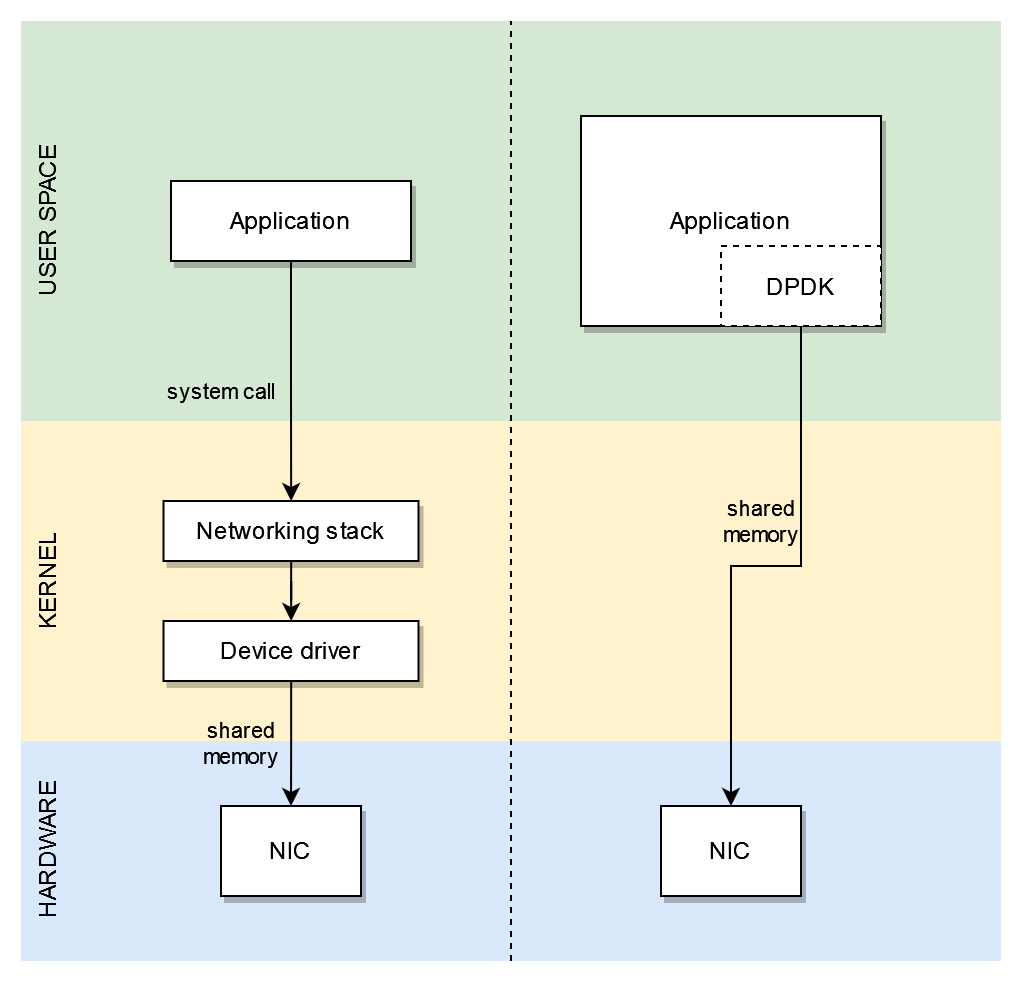
\includegraphics[width=0.7\textwidth]{graphics/trad-vs-dpdk.png}
    \caption{Data path monolitico vs DPDK}
    \label{fig:trad-vs-dpdk}
\end{figure}

Lo scenario descritto è adatto alla maggior parte degli usi: esso consente infatti di non sprecare cicli di clock con attese attive favorendo efficienza, risparmio energetico ed esponendo un'API semplice (le system call) uguale per ogni applicazione. Un elemento di rete però non è fatto per stare a riposo: sulle sue interfacce è logico trovare sempre traffico e deve dunque essere progettato focalizzandosi sulle alte prestazioni. L'alto livello di integrazione e il numero finito di funzioni che esso implementa consentono inoltre di rinunciare a qualche punto di flessibilità in favore delle performance.

Da queste idee è nata DPDK, una libreria per sviluppare applicazioni di networking in grado di gestire efficacemente un throughput molto elevato, nell'ordine di centinaia di Gigabit per secondo. Gli ingredienti fondamentali sono semplici:

\begin{itemize}
    \item Bypassare il kernel, permettendo alla scheda di rete di interagire direttamente con la memoria del processo
    \item Spostare i driver in user space, all'interno della libreria stessa
    \item Superare il modello interrupt-driven
\end{itemize}

La prima grande differenza rispetto all'approccio tradizionale è che in DPDK tutto ruota attorno al \textit{poll-mode driver} (PMD): non si usano gli interrupt in favore di una busy wait di nuovi dati in arrivo. Potrebbe sembrare un controsenso, ma ciò consente di incrementare notevolmente il packet rate poiché non si verificano più context switch legati alla gestione degli interrupt e la pipeline della CPU rimane a regime. Il dispositivo di rete quindi scrive i dati in arrivo direttamente in un'area di memoria precedentemente allocata e fissata (pinned) dal processo, il quale consuma gli stessi senza intermediari. 

Sul piano architetturale, trovano spazio i driver per un sott'insieme selezionato di device supportati, uno strato software di astrazione simile all'\textit{hardware abstraction layer} di tutti i principali sistemi operativi, timer e strutture dati, funzioni per l'accelerazione hardware come crittografia o QoS e poco altro. Questi componenti hanno la funzione di interfacciarsi col dispositivo, uniformandone il funzionamento ad alto livello, ed espletare quei compiti che normalmente ricadono sul kernel.

\begin{figure}[htb]
    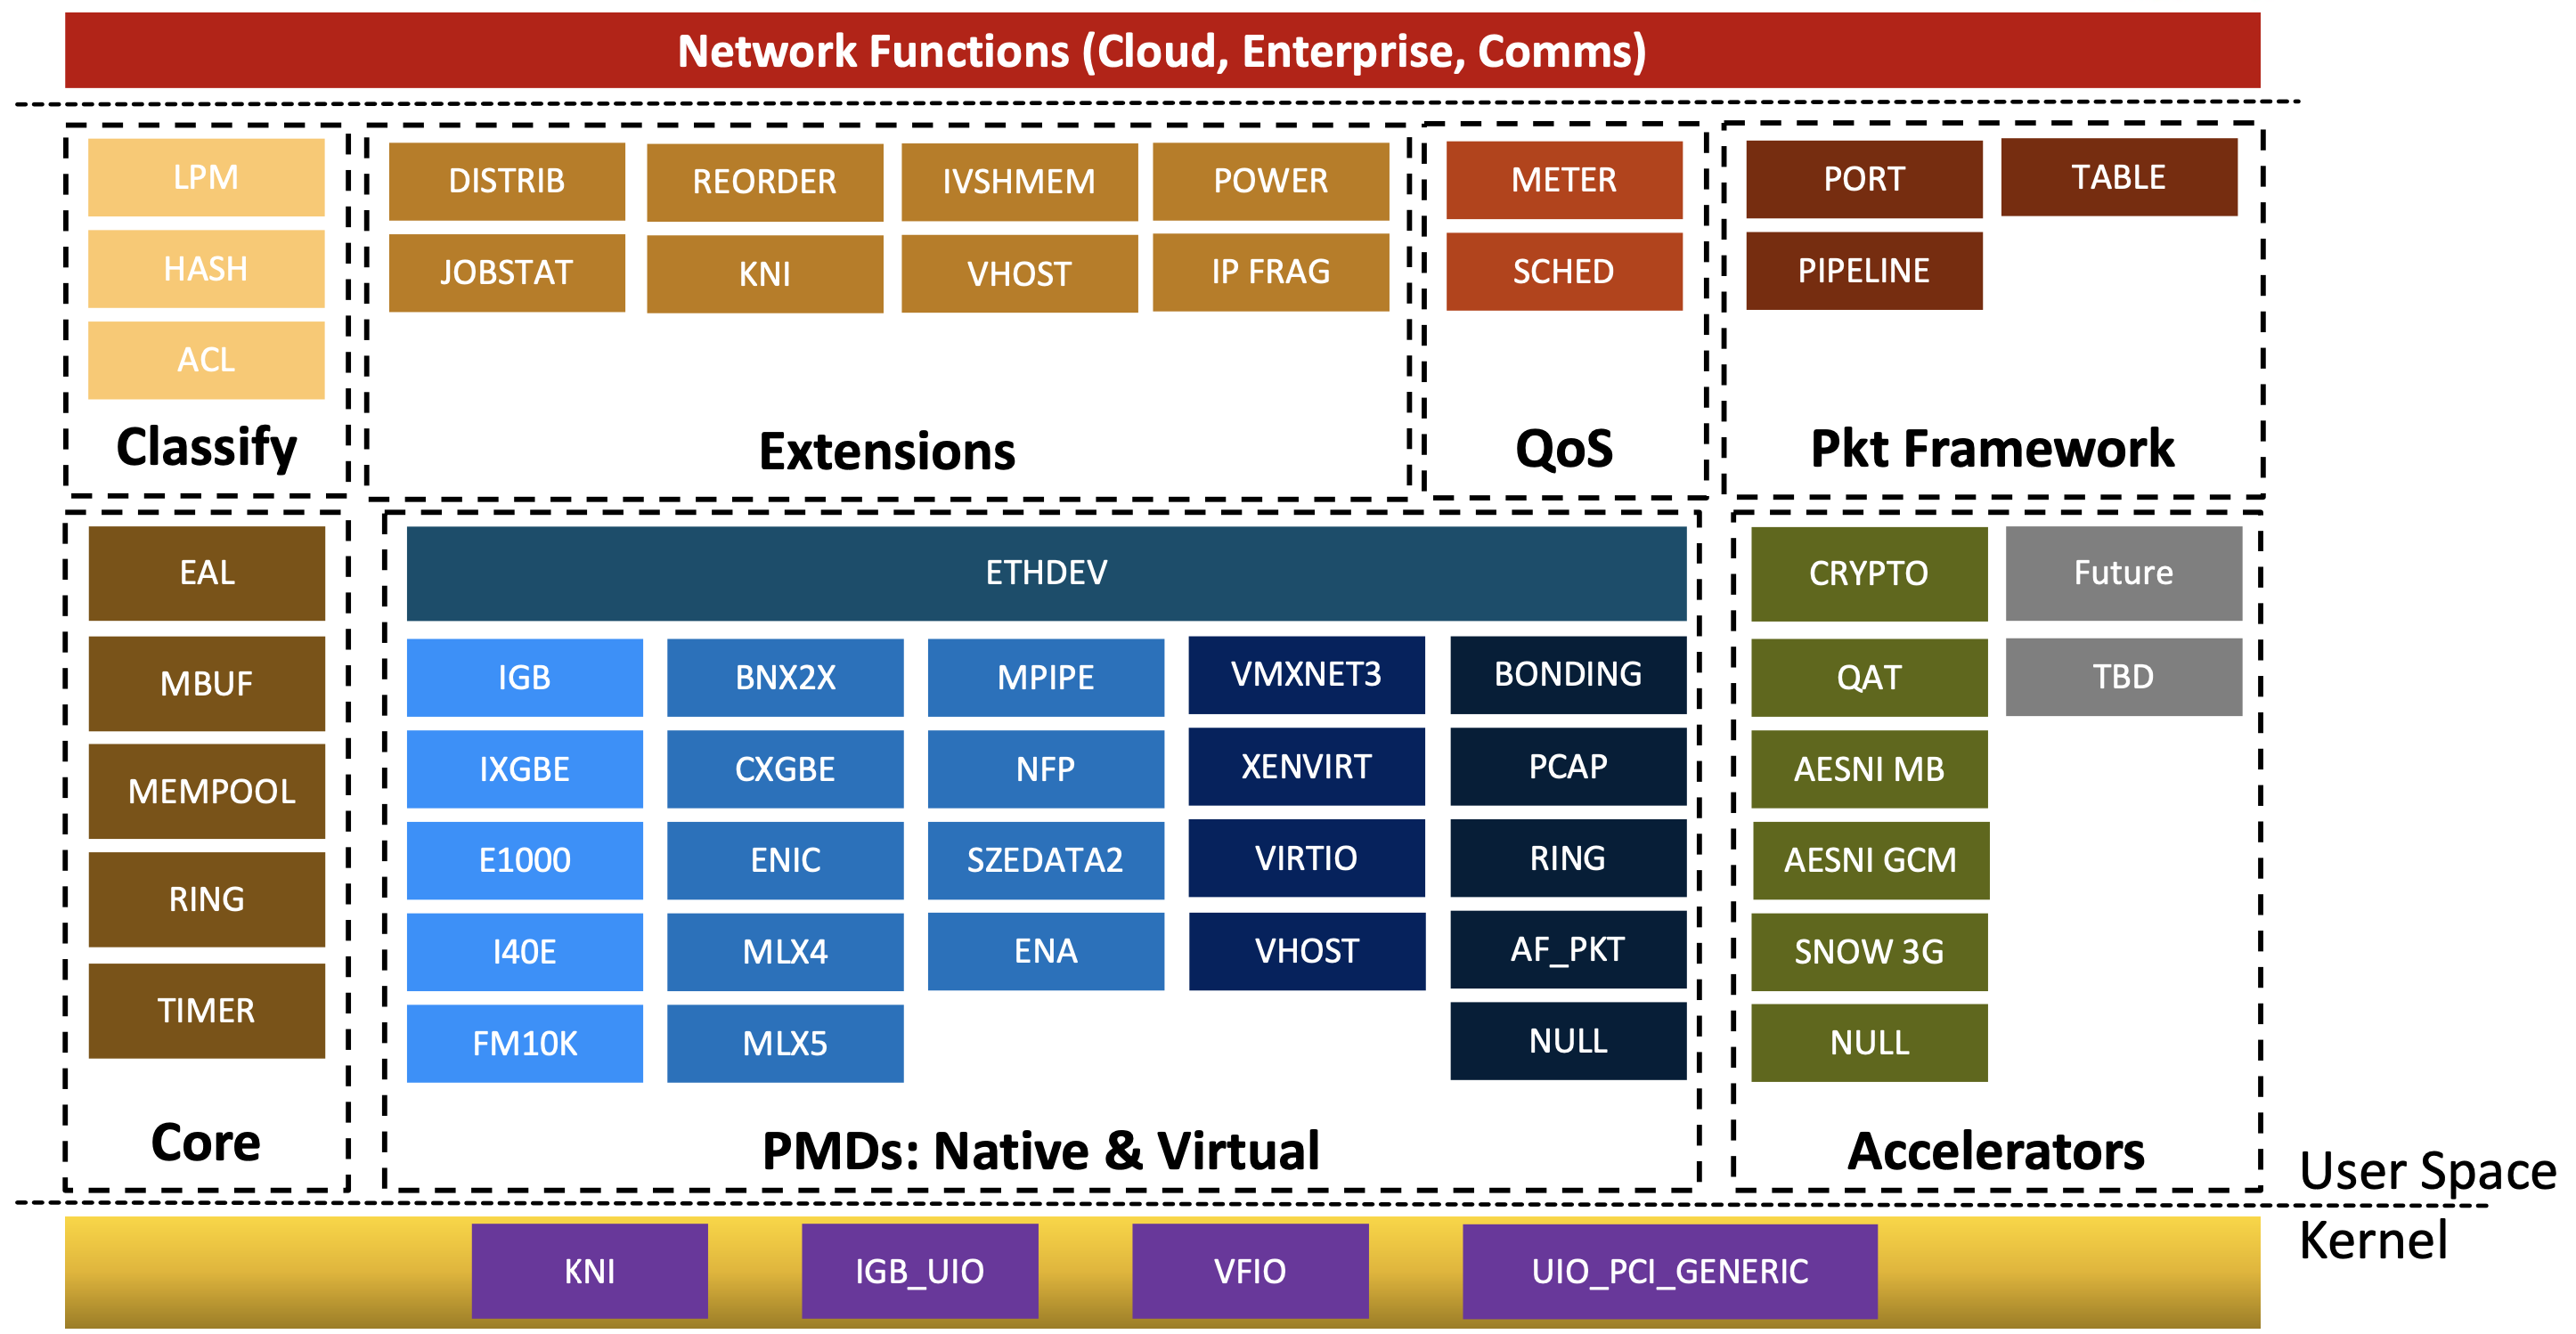
\includegraphics[width=0.8\textwidth]{graphics/dpdk-framework.png}
    \caption{DPDK Framework \cite{dpdk-intro}}
    \label{fig:dpdk-framework}
\end{figure}

Dal punto di vista teorico, DPDK realizza un \textit{exokernel}, ossia una tipologia di sistema operativo in cui il controllo dell'hardware è demandato direttamente ai programmi che ne fanno uso, mentre il nucleo ha la sola funzione di garantire l'accesso esclusivo ai dispositivi da parte dei vari processi. Anche in DPDK infatti quando un'applicazione assume il controllo di un'interfaccia questa diventa non più visibile al resto del sistema.

Nel corso della tesi si illustreranno alcuni usi di questo framework, principalmente legati al routing o al traffic generation, ma DPDK trova spazio anche nelle reti 5G a bassa latenza, nei firewall, in orchestratori come OpenStack o Kubernetes, in ambito HPC e in generale in tutti quei contesti dove il networking ad alte prestazioni è una prerogativa imprescindibile.

\section{VPP}
\label{sec:vpp}

Il paragrafo precedente descrive come DPDK assolva i compiti di un device driver, permettendo al software di dialogare con l'hardware in maniera efficiente grazie all'introduzione del poll-mode driver in user space. Il prossimo tassello dello stack tecnologico è rappresentato dal data plane. Anche in questo caso, trattandosi di un'architettura interamente virtualizzata e senza un particolare supporto hardware dedicato, entra in scena una libreria, frutto del lavoro di Cisco, open source e votata alla velocità.

L'intuizione fondamentale dietro VPP, acronimo di \textit{Vector Packet Processing}, è quella di sfruttare al massimo la pipeline delle moderne CPU scalari, operando su insiemi di dati piuttosto che pacchetti singoli al fine di ottimizzare l'utilizzo delle cache. Analogamente a quanto descritto nel paragrafo su DPDK, i pacchetti devono attraversare una serie di ``stazioni'' durante la loro elaborazione, ciascuna delle quali svolge una funzione precisa, come decodificare un header o interrogare una tabella d'inoltro.

\begin{figure}[htb]
    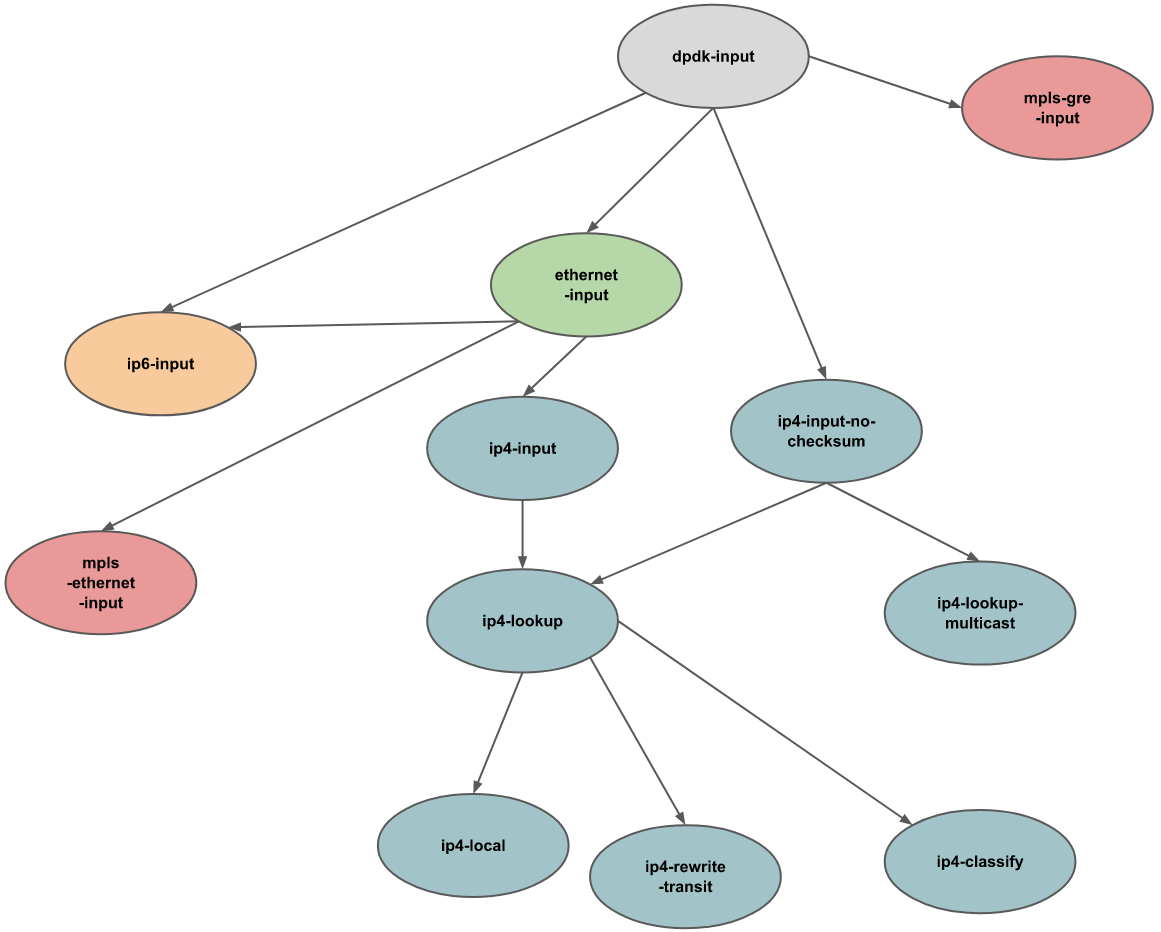
\includegraphics[width=0.7\textwidth]{graphics/vpp-dag.png}
    \caption{Il grafo diretto aciclico di VPP (estratto) \cite{vpp-overview}}
    \label{fig:vpp-dag}
\end{figure}

In VPP queste operazioni sono descritte da un grafo diretto aciclico (DAG) che definisce il flusso dei pacchetti sul data plane. La soluzione di Cisco però si differenzia nell'approccio. Nei sistemi operativi tradizionali, ogni pacchetto attraversa individualmente la pipeline di processing. Sommariamente, questo si traduce nei seguenti passi:

\begin{itemize}
    \item Load del pacchetto dati
    \item Load delle istruzioni inerenti una stazione di elaborazione
    \item Processing vero e proprio
    \item Load delle istruzioni inerenti la successiva stazione di elaborazione
    \item Processing
    \item ...
\end{itemize}

Le operazioni di load in particolare sono onerose in termini di cicli di clock, poiché richiedono importanti trasferimenti dalla memoria. VPP mira a risolvere questa criticità operando su \textit{vettori} di pacchetti piuttosto che singole unità. Se infatti la latenza di memoria dovuta al recupero delle istruzioni è inevitabile, una volta che queste hanno raggiunto la instruction cache della CPU possono essere riapplicate a molteplici dati della stessa natura aumentando l'efficienza in termini di pacchetti per secondo tanto più aumenta la dimensione del vettore. Parallelamente i pacchetti vengono caricati nella data cache in blocco, avvantaggiati dalle funzioni di load speculative delle moderne microarchietture. Applicando simultaneamente queste due ottimizzazioni, si riescono a ridurre significativamente i cache miss sia sulle istruzioni, poiché queste vengono riapplicate in serie per $N$ pacchetti, che sui dati, trasferiti a scaglioni, risultando in un incremento fino a 4-5 volte del numero di pacchetti elaborati al secondo da un singolo core.

Si tratta quindi di rovesciare il punto di vista quando si elaborano i pacchetti ragionando per livelli come meglio chiarito nella \cref{fig:scalar-vs-vector-packet-processing} invece che per unità. Ciò acquista maggior significato se si tiene conto dei pochi compiti in capo al data plane, che al più può incapsulare o decapsulare tunnel di varia natura, inoltrare pacchetti su interfacce diverse e tradurre indirizzi. Inoltre, risiedere in user space permette una sensibile flessibilità in fase di sviluppo e adozione di nuove funzionalità, così come consente un agile recupero in caso di errore: un'applicazione può essere riavviata senza troppi problemi, mentre un eventuale crash del kernel sarebbe catastrofico. Discorso analogo vale per gli aggiornamenti.

\begin{figure}[htb]
    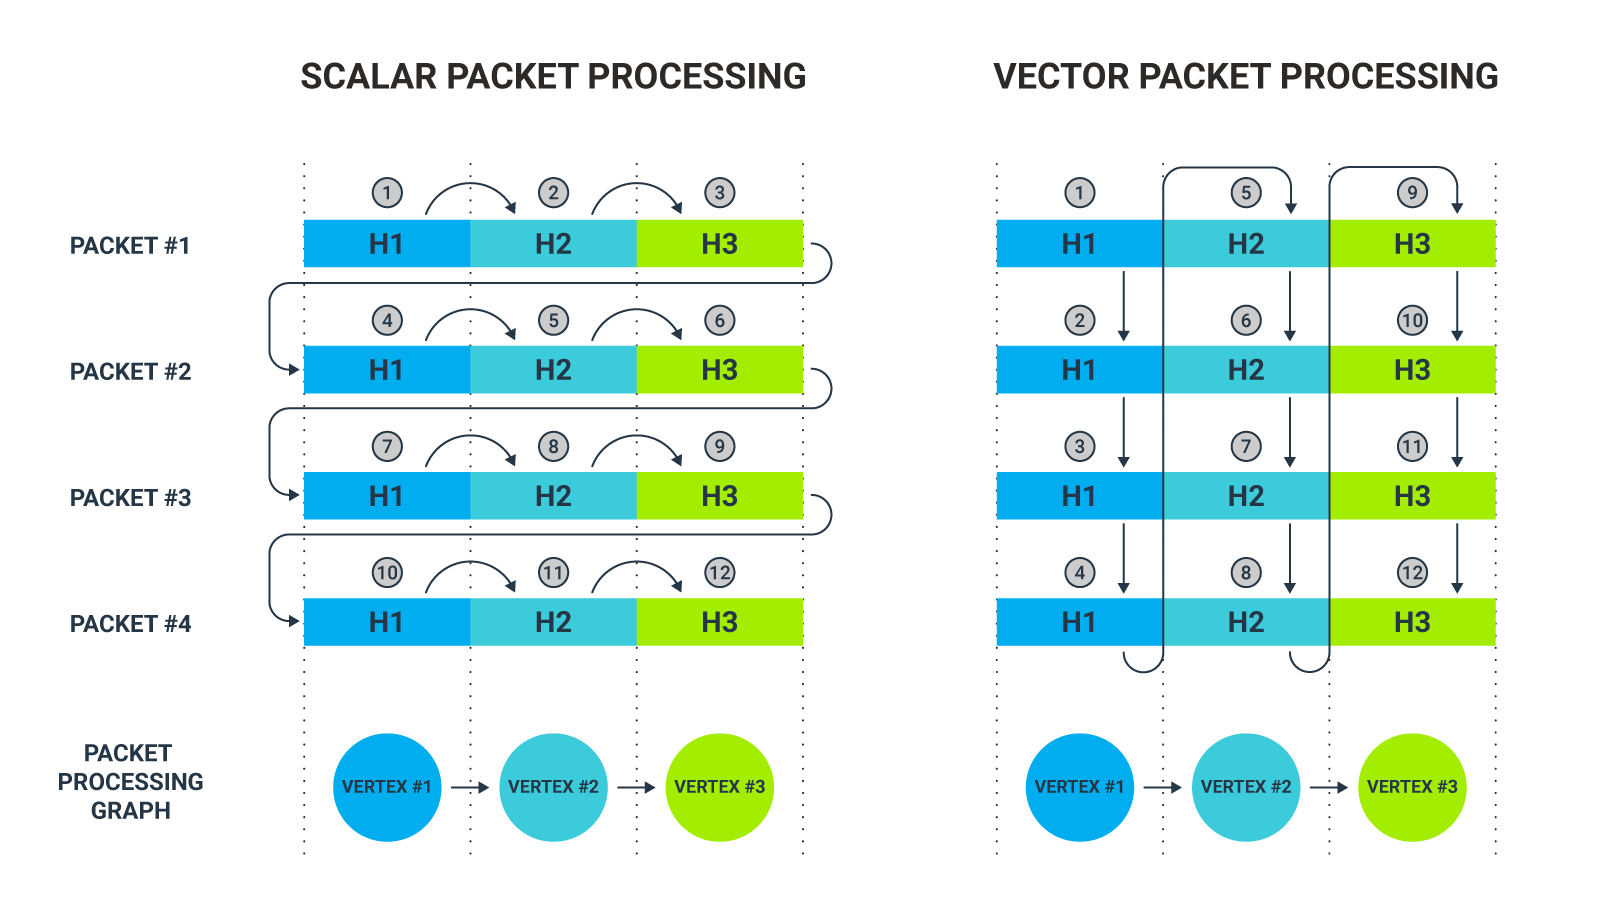
\includegraphics[width=0.8\textwidth]{graphics/codilime_scalar_packet_processing_vs_vector_packet_processing.png}
    \caption{Processing unitario (scalare) vs vettoriale}
    \label{fig:scalar-vs-vector-packet-processing}
\end{figure}

Come DPDK, anche VPP è passato sotto l'ombrello della Linux Foundation confluendo nel \textit{Fast Data Project} (FD.io). A livello architetturale, DPDK costituisce l'input per VPP e spesso quest'ultimo incorpora il primo come dipendenza software nelle vesti di plug-in (v. \cref{fig:vpp-dag} ``dpdk-input''). Trattandosi di componenti software, infine, entrambe si prestano ad applicazioni di vario genere, adattandosi facilmente a molti scenari cloud come macchine virtuali e container.

\section{FRRouting}

DPDK e VPP forniscono quanto necessario per realizzare un data plane software ad alte prestazioni, formando una sorta di ASIC virtuale. Chiave di volta per rendere operativa questa infrastruttura è un control plane in grado di istruire il piano d'inoltro nelle sue funzioni vitali e coordinarsi con gli altri apparati della rete per dirigere il traffico.

Entra dunque in scena \textit{Free Range Routing}, l'ultimo e forse più semplice elemento di questa architettura interamente virtuale. Nato come fork di Quagga, a sua volta derivato dall'ormai abbandonato GNU Zebra, FRRouting è un software libero composto da una collezione di demoni che implementano i più comuni protocolli del control plane oggi utilizzati. Al suo interno troviamo il trittico BGP/OSPF/IS-IS che nelle sue varie declinazioni domina il panorama intra- ed inter- sistemi autonomi, ma anche protocolli dedicati al multicast come PIM e IGMP, LDP per la distribuzione delle etichette MPLS, EVPN ed altri.

\begin{figure}[htb]
    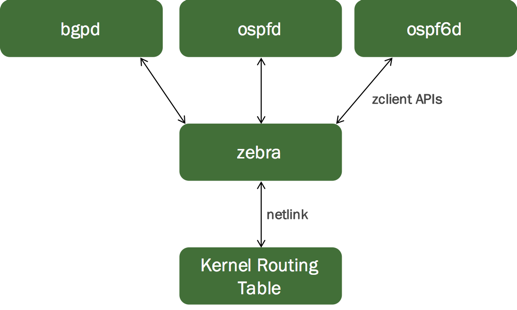
\includegraphics[width=0.7\textwidth]{graphics/frrouting-overview-daemons.png}
    \caption{Architettura di Free Range Routing}
    \label{fig:frr-arch}
\end{figure}

Il design è caratterizzato da una topologia master/slave (\cref{fig:frr-arch}) al cui centro trova spazio il demone principale, \textit{zebra}. Questo svolge il ruolo di accentratore per le informazioni provenienti dalle varie altre entità e si occupa di interfacciarsi col sistema operativo tramite \textit{netlink}, un protocollo di sistema aperto per la gestione delle interfacce di rete e del data plane.

Nei paragrafi precedenti è stato illustrato come DPDK e VPP si siano evoluti seguendo una filosofia bottom-up, ossia costruendo via via gli elementi necessari e astraendo il funzionamento dei livelli sottostanti. FRR invece ha vissuto una storia diversa: affermatosi prima dell'avvento di queste soluzioni innovative, ha sempre vissuto comodamente sopra qualunque tipo di sistema operativo senza richiedere particolari risorse. Sono state proprio la sua completezza e stabilità a renderlo il compendio ideale del panorama virtuale, tanto che nel giro di un paio d'anni sono stati fatti molteplici tentativi per integrarlo con lo strato superiore di VPP\footnote{\ La già citata Southbound API della \cref{sec:sdn-nfv}}. L'ultimo nonché l'unico ad aver avuto abbastanza successo da essere supportato nativamente si chiama \textit{linux-cp}, acronimo di ``Linux Control Plane'', ed è stato descritto dall'autore in una serie di articoli \cite{pim-linux-cp}. Il concetto è semplice: creare un'interfaccia virtuale gemella di quella fisica nel sistema operativo su cui VPP possa riversare tutto il traffico diretto specificatamente al router e mantenerne la configurazione allineata a quella interna. Ciò non costituisce un problema poiché la maggior parte dei pacchetti che attraversano un router sono solitamente ``di passaggio'', senza essere destinati all'apparato stesso, e quindi non lasceranno mai il data plane. I pochi restanti invece possono migrare da un dominio all'altro in maniera trasparente, beneficiando di tutto il software e la logica già comunemente presenti e senza reinventare la ruota.

All'atto pratico, \textit{linux-cp} è anch'esso un plug-in, un nodo del grafo diretto aciclico di VPP, ed è logicamente suddiviso in due parti:

\begin{enumerate}
    \item \textbf{Interface Mirror} che si occupa della sincronizzazione VPP \textrightarrow\ Linux
    \item \textbf{Netlink Listener} il cui compito è rimanere in ascolto dei messaggi \textit{netlink} in arrivo dal livello applicativo e apportare le dovute modifiche alla coppia di interfacce
\end{enumerate}

Grazie a Netlink e a \textit{linux-cp} è possibile collegare FRRouting al data plane evoluto VPP/DPDK (\cref{fig:tnsr-arch}) seguendo una metodologia top-down. Il plug-in permette inoltre di sfruttare tutti i classici strumenti come \textit{ping} e \textit{traceroute} sopra al nuovo stack senza necessità di modifiche.

\section{TNSR}

I tre paragrafi precedenti introducono i pilastri del routing interamente softwarizzato, di cui rappresentano lo stato dell'arte. Combinarli però non è banale: si rischiano incompatibilità e colli di bottiglia difficili da scovare. Per questo motivo Netgate ha creato TNSR, una distribuzione di Linux basata su Ubuntu\footnote{\ Precedentemente si basava su CentOS, con differenze minime} che presenta un ambiente preconfigurato simile ad un router commerciale. L'azienda, già famosa per aver creato pfSense, un firewall virtuale open source molto apprezzato, è impegnata nel contribuire all'ecosistema con l'obiettivo di rafforzarlo e renderlo più adatto ad un uso reale, intravedendo in TNSR uno step intermedio verso un firewall ad alte prestazioni.

Peculiarità di TNSR è la suddivisione in namespace. Linux mette a disposizione questa tecnologia per favorire l'isolamento dei processi e delle risorse, di fatto la base della cosiddetta ``OS-level virtualization'', comunemente nota come \textit{container}. Nella fattispecie, TNSR usa due distinti networking namespaces per il router ed il management plane: il primo, chiamato ``dataplane'', contiene lo stack VPP/DPDK, la suite FRR e Strongswan per la gestione dei tunnel IPSec, mentre nel secondo si trovano la CLI, il server SSH per l'accesso remoto, il database delle configurazioni e altri strumenti utili alla gestione del router e del suo sistema operativo.

\begin{figure}[htb]
    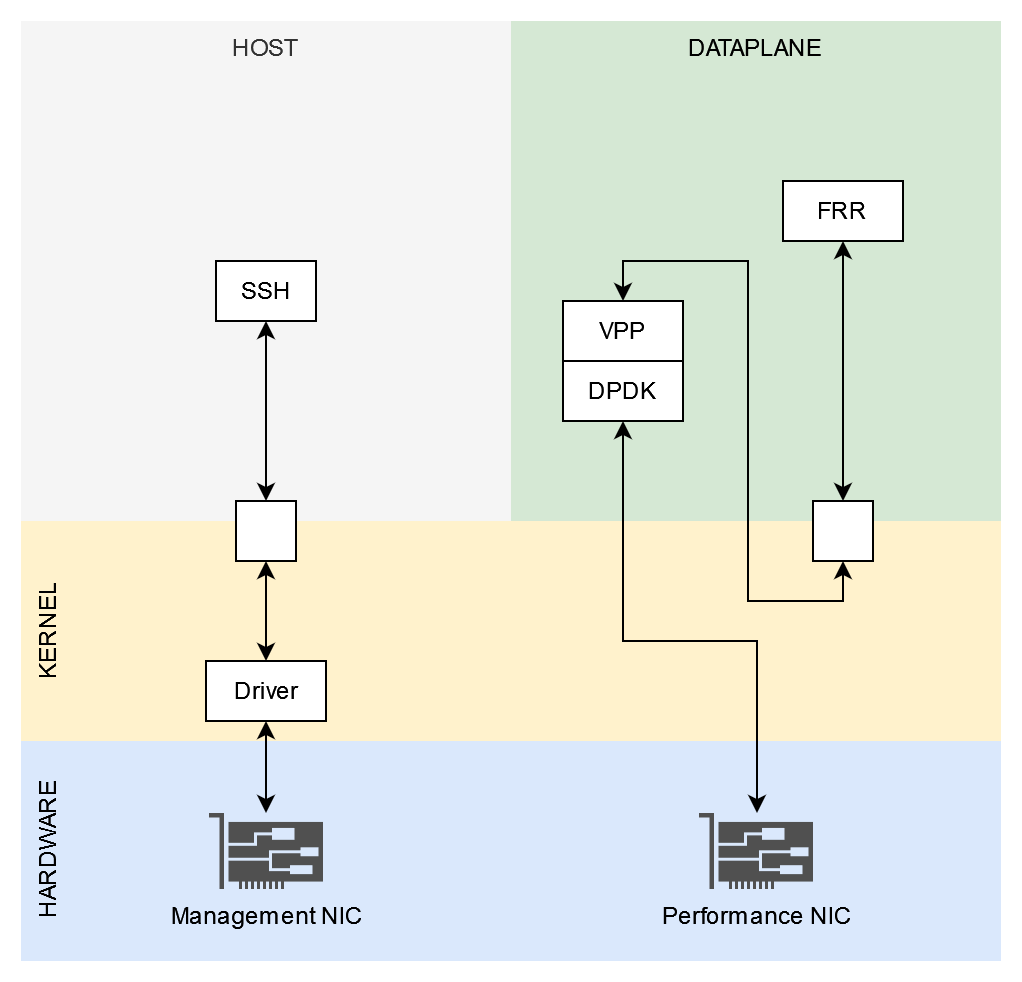
\includegraphics[width=0.7\textwidth]{graphics/tnsr-arch.png}
    \caption{Architettura di TNSR (estratto)}
    \label{fig:tnsr-arch}
\end{figure}

Separare i due ambienti in questo modo offre svariati vantaggi: in primo luogo previene che malfunzionamenti in una o nell'altra parte possano ripercuotersi sull'operatività generale del router, potendo ad esempio disporre di un'entrata di management anche in caso di errori di configurazione del dataplane. Inoltre, siccome i dispositivi di rete così come i processi sono isolati all'interno di ciascun namespace, non si rischia confusione durante l'assegnazione delle interfacce che possono essere acquisite automaticamente dai rispettivi stack di rete. Anche le tabelle di inoltro sono diverse, fattore che contribuisce alla sicurezza generale e all'affidabilità della soluzione. Ultimo ma non meno importante, testimonia come queste tecnologie possano funzionare all'interno di container, caratteristica che ne aumenta l'appetibilità col passare del tempo. Non sorprenderebbe se in futuro questi software raggiungessero un livello di maturità tale da essere orchestrati su cluster di container all'edge della rete. Oggi tuttavia la tecnologia è ancora acerba: manca ad esempio la possibilità in orchestratori come Kubernetes di definire la presenza di una certa scheda di rete come requisito. Alcuni plug-in promettono di estenderne le funzionalità, ma non sembrano attrarre particolare interesse, almeno per il momento. Virtualizzatori come Proxmox, invece, già consentono di eseguire container al pari di macchine virtuali, ma così facendo verrebbe meno la parte di resilienza, fallback e load balancing automatici.

È opinione di chi scrive che la semplice architettura di TNSR, elegante e funzionale, tornerà a far parlare di sé in futuro, venendo rivisitata in altre applicazioni simili per mezzi, ma diverse per finalità.

% https://m.facebook.com/NetgateUS/posts/10155790595267689

\section{DANOS}

Finora si è parlato di stack completamente virtuali, senza l'ausilio di acceleratori hardware legati a funzionalità specifiche. Questo approccio è generalmente preferibile quando si ha a che fare con funzioni diverse e complesse quali ad esempio certe componenti dell'architettura LTE. Nel caso del puro forwarding invece è difficile raggiungere throughput importanti senza circuiti dedicati: nonostante molti studi e gli esperimenti che verrano discussi nel \cref{chap:lab} suggeriscano che la suite VPP/DPDK scali linearmente all'aumentare della potenza di calcolo, permangono limiti fisici, tecnologici ed economici che ne scoraggiano l'utilizzo in condizioni di traffico molto elevato come la rete core di un grande provider.

Queste ragioni hanno guidato lo sviluppo di una nuova classe di dispositivi, i \textit{whitelabel switch}. Si tratta in sostanza di router e switch simili agli apparati tradizionali, ma privi di sistema operativo. A realizzarli sono spesso aziende nuove del settore, case come Broadcom, specializzata in chip, che decidono di cimentarsi nell'impresa di produrre processori dedicati, chiamati \textit{network processing unit} o più sovente \textit{merchant silicon}, e di venderli ad altre realtà affinché possano produrre soluzioni complete. Diversamente dai vendor verticalmente integrati, questa famiglia è caratterizzata da ASIC programmabili e quindi facilmente customizzabili tanto che si stanno affermando nuovi linguaggi di programmazione specificatamente orientati all'implementazione di nuovi protocolli del data plane, tra cui \textit{P4}.

DANOS è un sistema operativo disaggregato e aperto per apparati di rete \cite{danos-whitepaper}. Il suo obiettivo non è realizzare una soluzione completamente softwarizzata, ma piuttosto di essere in grado di dialogare con qualunque tipo di data plane, fisico o virtuale. Contiene dunque al suo interno i driver necessari ad interfacciarsi con l'hardware specializzato sottostante per l'offload di task specifici realizzando di fatto una Southbound API verso il \textit{merchant silicon}. Anche il control plane nasce con l'intento di essere modulare, potendo spaziare da un edge router ad un gateway per la telefonia mobile.

Il progetto è ancora acerbo, l'immagine aperta pubblicata contiene un data plane basato su DPDK e derivato da quello di Vyatta, un altro famoso router virtuale costruito su Linux. Vista la natura sperimentale, è probabile che alcune grandi aziende ne usino internamente versioni customizzate per i propri fini. Dal 2018 è entrato a far parte anch'esso della Linux Foundation, ma la community è poco attiva e l'entusiasmo iniziale sembra scemato. Forse in futuro, col progresso della tecnologia e dei whitelabel switch, se ne sentirà di nuovo parlare, ma resta un buon esempio delle molteplici iniziative di networking aperte ed interoperabili nonché dei diversi approcci saggiabili nel settore.

\section{XDP}

Parallelamente alla nascita di DPDK, altre tecnologie vedevano la luce tra cui \textit{eXpress Data Path} (XDP): una ``scorciatoia'' nel kernel Linux introdotta nella versione 4.8 \cite{xdp-paper}. Nei paragrafi precedenti si è discusso come DPDK scelga la strada radicale di bypassare in toto il kernel, spostando tutto il processing in user space; al contrario XDP è più conservativo e si avvale di un filtro programmabile insito in Linux per effettuare alcune operazioni ``al volo'' prima che i pacchetti lascino il driver, prima ancora che il sistema operativo allochi i buffer necessari a contenerli.

Grazie una macchina virtuale chiamata \textit{extended Berkeley Packet Filter} (eBPF) e supportata dalla maggior parte dei driver di rete\footnote{\ Talvolta pure a bordo delle stesse NIC in modalità offload} è possibile scrivere un programma, sicuro by design, che prenda decisione sulla base di campi prefissati del pacchetto ed esegua alcune semplici azioni come:

\begin{itemize}
    \item \verb|DROP|, per scartare il pacchetto
    \item \verb|TX|, per ritrasmettre il pacchetto alla stessa scheda che l'ha ricevuto, eventualmente dopo averlo modificato
    \item \verb|REDIRECT|, per spostare il pacchetto su un'altra NIC o inviarlo ad un programma in user space tramite un socket \verb|AF_XDP|
    \item \verb|PASS|, per continuare la classica pipeline di elaborazione
\end{itemize}

\begin{figure}[htb]
    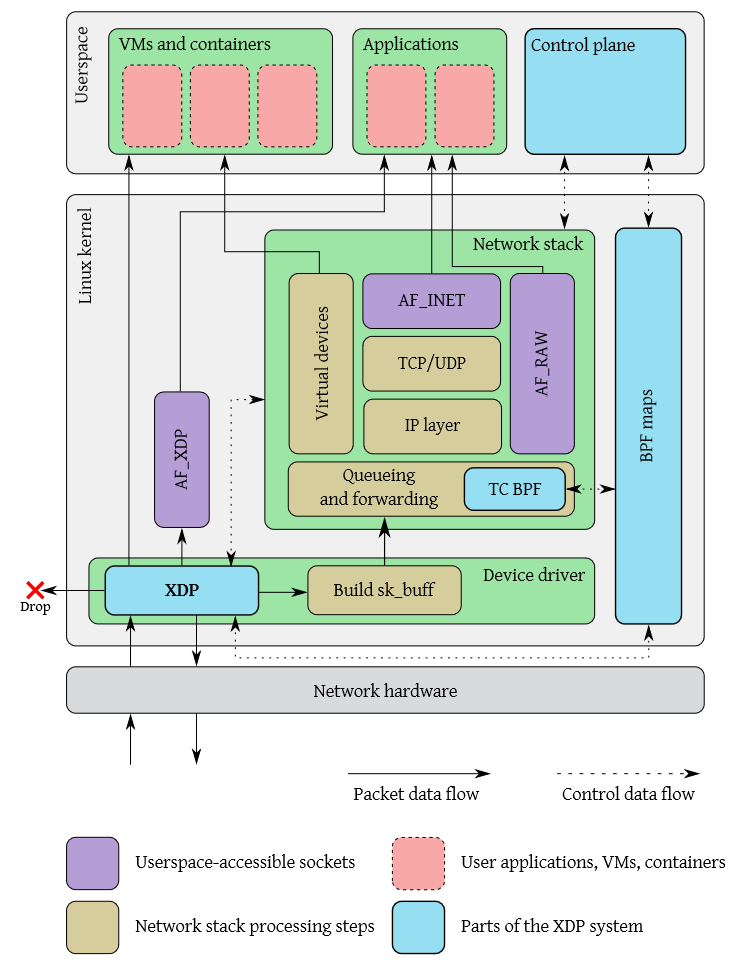
\includegraphics[width=0.7\textwidth]{graphics/xdp-datapath.png}
    \caption{Anatomia di XDP}
    \label{fig:xdp-datapath}
\end{figure}

Gli usi sono molteplici: la possibilità di passare i pacchetti allo user space o a delle macchine virtuali consente di implementare una funzione simile a quella dei controllori SDN per il traffico non classificato. Si può inoltre realizzare un router, tenendo però a mente che eventuali regole di firewall andrebbero reimplementate, in quanto normalmente situate più a valle nella pipeline di processing \cite{xdp-router-apnic}. In alternativa, questo tipo di filtro si presta molto bene alla mitigazione di attacchi di tipo DDoS, alleggerendo il sistema operativo dall'overhead dovuto al processing dei pacchetti malevoli \cite{cloudflare-ddos-xdp}.

Sul piano delle performance non può beneficiare dei vantaggi ``vettoriali'' di VPP, ma riesce ugualmente ad ottenere risultati sensibilmente superiori all'elaborazione tradizionale. Un altro tallone d'Achille è l'intrinseca limitazione: a partire da Linux 5.1 i programmi XDP sono limitati ad eseguire un milione di istruzioni\footnote{\ Prima erano solamente 4096!}, non potendo quindi ambire a task più complessi di un router o di un semplice packet filter.

\section{TRex}

Delle tante applicazioni di DPDK, una sicuramente degna di nota è TRex, un traffic generator L3-7 open source creato da Cisco. A differenza di altri prodotti commerciali, TRex non punta a creare traffico ex novo, ma si limita a replicare dei flussi di catture esistenti modificando i campi chiave dei pacchetti e potendo contare sull'alta efficienza di DPDK per invio e ricezione. Questa combinazione permette di raggiungere velocità nell'ordine di centinaia di Gigabit al secondo su un moderno laptop, abbattendo sensibilmente i costi legati a questo tipo di appliance. Il software presenta due principali modalità operative:

\begin{itemize}
    \item Stateless, adatto a testare apparati di livello 3 e tunnel, supporta fino a \mbox{10mila} stream paralleli e 30 milioni di pacchetti al secondo per core e permette di misurare latenza e jitter dei pacchetti
    \item Stateful, in grado di emulare un protocollo livello 7, ottimo per mettere alla prova NAT, firewall, load balancer ed altri applicativi che si avvalgono della cosiddetta \textit{Deep Packet Inspection} (DPI)
\end{itemize}

A livello hardware, supporta tutte le schede di rete supportate da DPDK, \eng{device} virtualizzati, SR-IOV ed è possibile eseguirlo dentro un container. Ovviamente, perché raggiunga il massimo delle potenzialità, sono necessarie alcune accortezze legate al discorso NUMA che verranno meglio affrontate nel \cref{chap:lab}, ma tramite la configurazione guidata molti passaggi vengono espletati in automatico.
  \chapter{Virtualizzazione}
\label{chap:virt}

Quanto descritto nel capitolo precedente costituisce il livello più alto dell'architettura NFV, le \textit{Virtualized Network Functions} (VNFs). In particolare, si descrive il software in grado di svolgere una determinata funzione virtuale: il router. Queste pagine invece si pongono l'obiettivo di fornire una panoramica in cui inquadrare lo strato infrastrutturale, presentando alcune tecnologie fondazionali di virtualizzazione e tratteggiando il ruolo dell'orchestratore.

\section{SR-IOV}

Parlando di DPDK si è dato per scontato che una scheda di rete potesse essere assegnata ad una VNF senza problemi e senza overhead. In effetti i moderni hypervisor consentono di destinare un intero device ad una macchina virtuale o ad un container, nel primo caso con un'operazione detta ``PCI Passthrough'', nel secondo spostando il dispositivo nel namespace desiderato. Cosa succede però se una stessa interfaccia deve essere assegnata a più entità, scenario comune nelle architetture complesse? La soluzione solitamente consiste nel creare un bridge, ossia uno switch virtuale in kernel che emuli più NIC virtuali sopra una sola fisica, vanificando però le ottimizzazioni in capo a DPDK.

\begin{figure}[htb]
    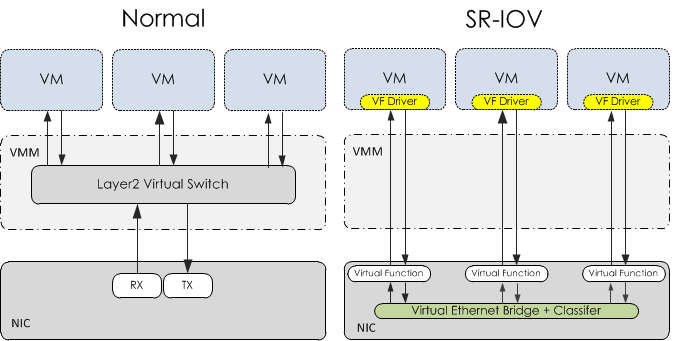
\includegraphics[width=0.7\textwidth]{graphics/sriov_overview.png}
    \caption{Bridge virtuale vs SR-IOV}
    \label{fig:sriov-overview}
\end{figure}

Single Root I/O Virtualization (SR-IOV) è una funzionalità di PCI Express Extended che permette ad un dispositivo fisico di apparire come più dispositivi virtuali. Il dispositivo fisico è denominato \textit{Physical Function} (PF) mentre i dispositivi virtuali sono chiamati \textit{Virtual Functions} (VF). Grazie a SR-IOV è possibile accedere a ciascuna funzione virtuale tramite un indirizzo PCIe univoco. Ogni device virtuale ha il proprio spazio di memoria PCI, che viene utilizzato per mappare il suo set di registri ed il driver del dispositivo virtuale opera su di essi al pari di uno fisico, mascherando l'astrazione al sistema operativo.

Nel caso delle schede di rete, ogni interfaccia è dotata di un proprio indirizzo di livello 2 (MAC) e di buffer in ricezione ed invio dedicati. Il bridging prima effettuato dal kernel viene adesso svolto dal microcontrollore a bordo della scheda di rete. Una NIC che supporti DPDK ed SR-IOV è dunque in grado di essere assegnata contemporaneamente a più VNFs senza comprometterne le performance ed in maniera trasparente.

Spostare lo switch virtuale verso il dispositivo fisico ha però lo svantaggio di allungare il percorso quando i pacchetti sono destinati ad una VNF sullo stesso server di quella mittente, occupando il bus PCI inutilmente. Alcuni studi recenti aprono alla possibilità di realizzare uno switch virtuale con DPDK (OVS-DPDK) e ipotizzano diverse tipologie di traffico: est-ovest per la comunicazione tra VNF nello stesso dominio, nord-sud altrimenti. I risultati dipendono molto dalla natura del traffico e non emerge un chiaro vincitore: uno switch virtuale basato su DPDK è preferibile in caso di pattern est-ovest, ma bisogna prestare attenzione al tipo di funzione che si vuole realizzare e se questa possa o meno trarre beneficio dall'uso di un approccio vettoriale come VPP. In tutti gli altri casi, si dimostra come SR-IOV scali linearmente all'aumentare di funzioni virtuali \cite{intel-sriov, cisco-sriov}.

\section{KVM}

Risalendo lo stack infrastrutturale, appena sopra l'hardware, troviamo il layer di virtualizzazione. Lo scopo di questo livello intermedio è quello di astrarre, partizionare e gestire le risorse fisiche del server potendone permettere l'assegnazione a più funzioni virtuali. Non si parla ancora di gestione federata, per adesso il focus è incentrato sul singolo host.

\textit{Kernel-based Virtual Machine} (KVM) è un modulo di Linux che trasforma il kernel in un hypervisor, rendendolo in grado di ospitare ed eseguire macchine virtuali, assegnando risorse come numero di core, quantità di memoria RAM e dispositivi fisici. In KVM, ogni CPU virtuale è mappata su un thread del sistema operativo, operazione necessaria a garantirne il corretto isolamento. Sopra i processori così realizzati viene eseguito il sistema operativo guest proprio della macchina virtuale e tutte le relative applicazioni.

\begin{figure}[htb]
    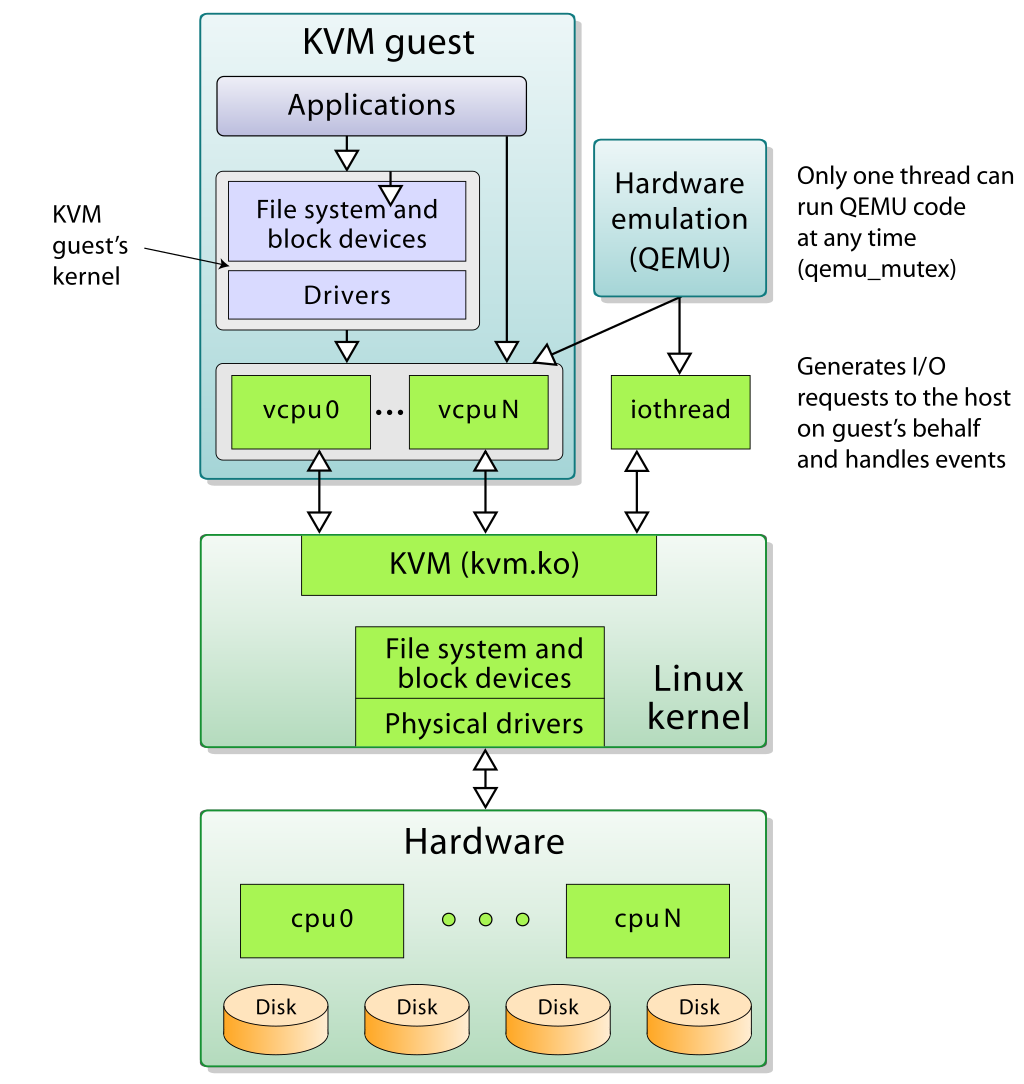
\includegraphics[width=0.7\textwidth]{graphics/kvm.png}
    \caption{Architettura di KVM}
    \label{fig:kvm-arch}
\end{figure}

Nello schema proposto in \cref{fig:sriov-overview} KVM è rappresentato dal \eng{Virtual Machine Monitor} (VMM) ed ha il compito di assegnare funzioni virtuali della NIC SR-IOV alle diverse VM, dando loro diretto accesso al bus PCI. Non è genericamente compito dell'hypervisor emulare dispositivi virtuali, motivo per cui KVM è spesso usato in accoppiata con un altro software: QEMU. Emulare un device via software ne riduce le performance e per questo si cerca di limitarne gli usi a quelle periferiche ``lente'' necessarie al corretto funzionamento delle macchine virtuali come mouse, tastiera e uscita video.

\section{NUMA}

I sistemi multi-CPU sono una realtà consolidata. La domanda di potenza computazionale cresce molto più rapidamente della capacità dei processori, inevitabilmente limitati dalla legge di Moore. Le architetture multicore sono complesse da progettare e la loro scalabilità limitata: mettere troppi core su un singolo chip non è possibile perché il segnale di clock impiegherebbe troppo tempo per propagarsi. Inoltre, il calore generato sarebbe eccessivo e i continui messaggi di aggiornamento delle cache condivise finirebbero col saturare la trama di interconnessione ed i core stessi.

L'alternativa è rappresentata dai sistemi multi-processore in cui più CPU identiche trovano spazio sulla medesima scheda madre e sono collegate da dei bus. L'organizzazione può essere di due tipi:

\begin{itemize}
    \item Tutti i processori vedono tutta la memoria indiscriminatamente e per questo vengono chiamati sistemi \textit{Uniform Memory Access} (UMA)
    \item Ciascuna CPU è direttamente connessa ad una porzione di memoria e può accedere al resto tramite le altre CPU, \textit{Non-Uniform Memory Access} (NUMA)
\end{itemize}

Le architetture UMA sono naturalmente le più semplici da progettare e da gestire, ma non sono le più efficienti. La memoria rischia di saturarsi velocemente sotto il carico di decine di core che eseguono operazioni di lettura e scrittura contemporaneamente, ponendo un serio limite alla scalabilità del sistema. Viceversa NUMA consente di sfruttare il principio di località dei dati e dei programmi, ridistribuendo il carico per aree. Lo svantaggio è che il sistema operativo ed il progettista devono tener conto del layout sottostante ed elaborare soluzioni ``NUMA-aware'' che ripartiscano il lavoro tra i processori e le memorie sulla base dei dati acceduti più frequentemente.

\begin{figure}[htb]
    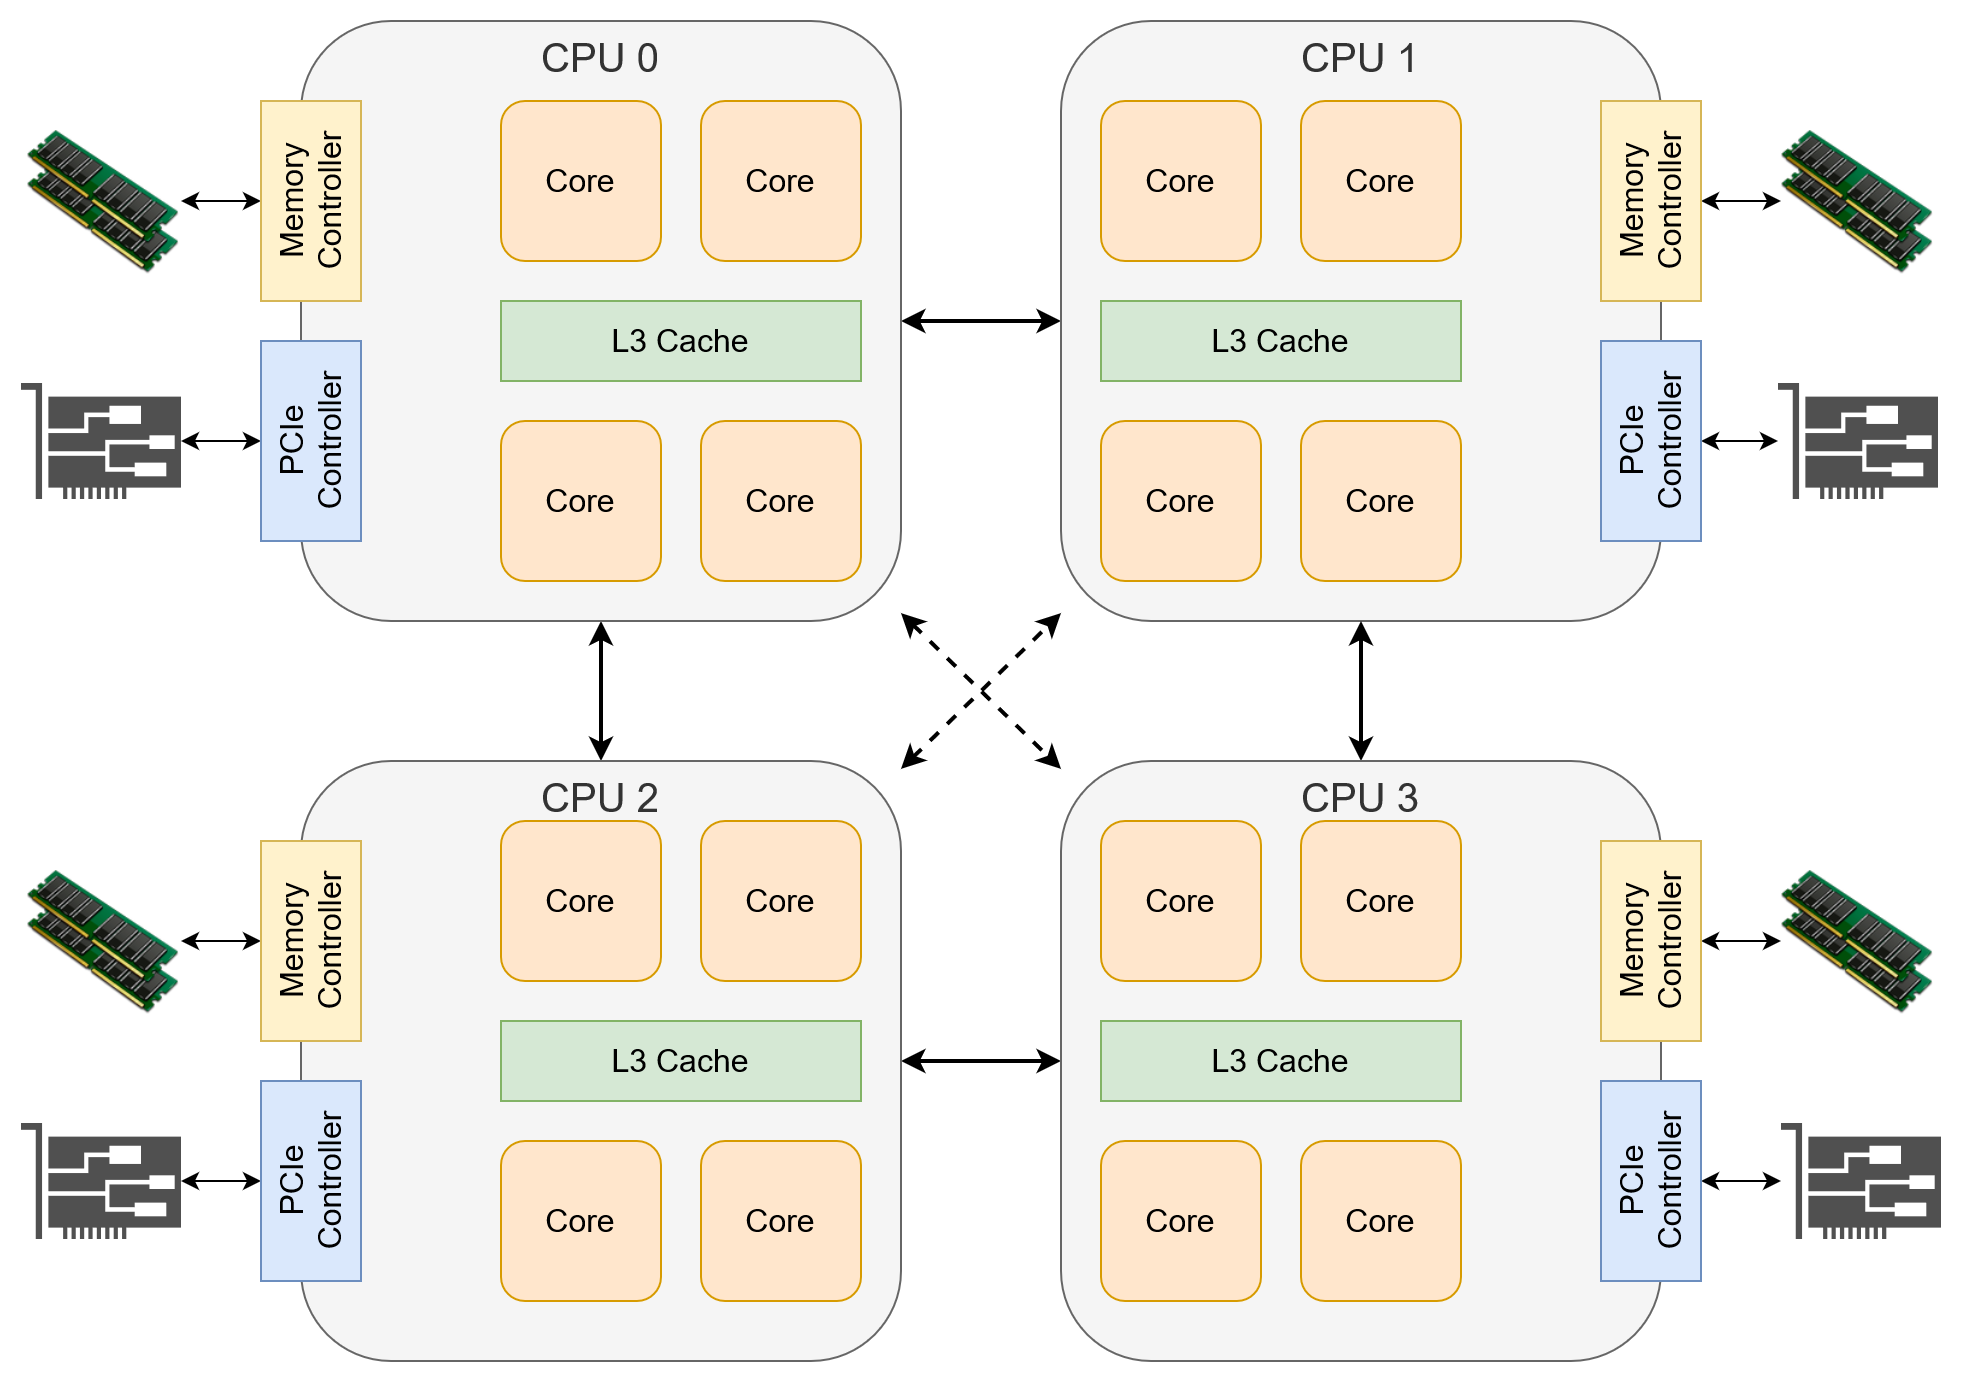
\includegraphics[width=0.8\textwidth]{graphics/numa.png}
    \caption{Layout NUMA}
    \label{fig:numa}
\end{figure}

Ciascun insieme di CPU, memoria e dispositivi direttamente connessi tra loro costituisce un ``nodo NUMA''. I nodi NUMA possono essere interconnessi in vari modi: singolo bus condiviso, anello, maglia completa,... in funzione delle potenzialità richieste e del prezzo. Per stimare il costo di passare da un nodo ad un altro, Linux usa una matrice delle distanze, una sorta di grafo che rappresenta la latenza nell'accedere ad una porzione di memoria: accedere alla propria memoria ha un valore di default pari a 10 mentre quello degli altri nodi dipende dal layout fisico.

Non solo la memoria, ma anche i dispositivi sono da tenere in considerazione: una scheda di rete direttamente connessa ad una CPU potrà minimizzare le latenze e massimizzare il throughput solo se il software con cui dialoga è fisicamente situato sullo stesso processore. Diversamente i dati dovranno attraversare la fabric di interconnessione cosa che nel complesso potrebbe avere ripercussioni pesanti su tutto il sistema.

Come discusso nel \cref{chap:lab}, un'allocazione ragionata delle VNFs che tenga conto della topologia sottostante può avere importanti benefici sulle performance, soprattutto in condizioni di elevato carico del server. Il progettista deve porre la dovuta attenzione nella definizione dei requisiti della VNF alla luce dei software che essa ospita e l'orchestratore dev'essere in grado di allocare le risorse di conseguenza.

\begin{figure}[htb]%
    \centering
    \subfloat[Accesso remoto]{{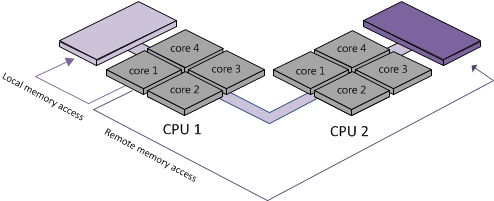
\includegraphics[width=0.45\textwidth]{graphics/numa-vm-1.png} }}%
    \qquad
    \subfloat[Pinning delle risorse]{{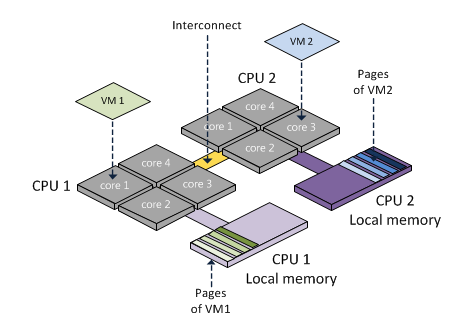
\includegraphics[width=0.45\textwidth]{graphics/numa-vm-2.png} }}%
    \caption{Esempi di allocazione NUMA-aware}%
    \label{fig:example}%
\end{figure}

\section{OpenStack}

Il paragrafo precedente descrive il ruolo del layer di virtualizzazione, centrale nella realizzazione dell'infrastruttura NFV (NFVI, \cref{fig:esti-nfv-low-level}). È bene ricordare che KVM non è l'unica possibile alternativa: come detto il framework ETSI NFV è agnostico rispetto alla tecnologia. Un hypervisor fine a se stesso però non è molto utile, serve un'infrastruttura in grado di gestire automaticamente centinaia se non migliaia di server con ancor più macchine virtuali e container.

Nell'ultimo decennio l'industria ha fatto passi da gigante in questa direzione, producendo gli \textit{orchestratori}, software in grado di far incontrare la disponibilità fisica di risorse con la domanda dei servizi, incastrando requisiti e funzionalità e fornendo altresì delle metriche relative all'esecuzione. In quest'ottica s'inserisce OpenStack, una piattaforma di cloud computing aperta e multi-vendor tra le più usate al mondo. Composto da una miriade di sotto-progetti che spaziano dal compute allo storage passando per load balancer, billing e monitoring, OpenStack è perfetto per assolvere le funzioni di NFVI e VIM (Virtualized Infrastructure Manager).

Tra i progetti di cui si compone, vi è Tacker, un modulo che implementa la parte alta di NFV MANO (VNF Manager e NFV Orchestrator) facendosi carico del ciclo vitale delle istanze VNF. La natura aperta di OpenStack lo rende facilmente interoperabile con altre soluzioni, tanto che chi non volesse usare Tacker può avvalersi di Open Source MANO per il macro-blocco di management e orchestration il quale dialoga con il livello infrastrutturale di OpenStack tramite la Northbound API.

\begin{figure}[htb]
    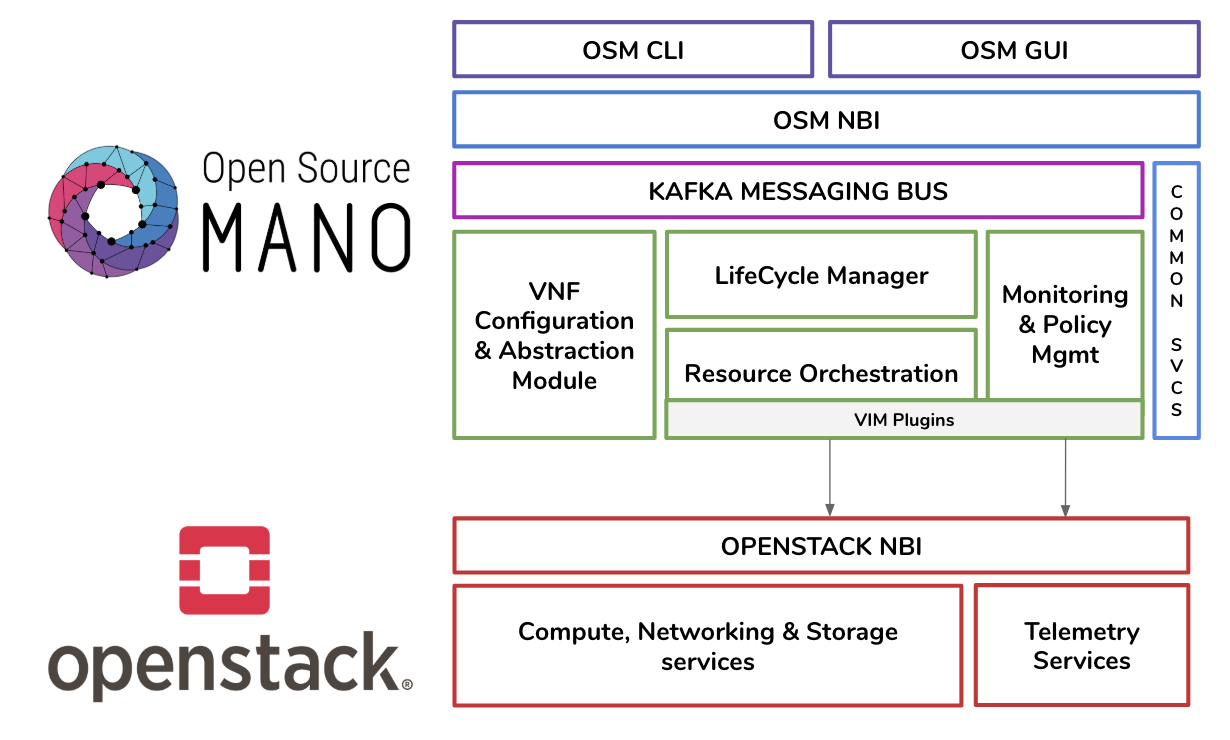
\includegraphics[width=0.7\textwidth]{graphics/openstack-mano.png}
    \caption{Northbound API tra OpenStack e Open Source MANO}
    \label{fig:openstack-mano}
\end{figure}

Vale la pena notare che ciascuno dei componenti qua citati è in realtà un software completo, costituito da vari servizi che segue un iter di sviluppo proprio. La complessità di tutte queste ``parti mobili'' ed il modo in cui esse interagiscono tra loro tramite API standard ricorda quella di un sistema operativo, tant'è che s'inizia a parlare di \textit{cloud operating system} o \textit{network operating system}.

% Tacker is an official OpenStack project building a Generic VNF Manager (VNFM) and an NFV Orchestrator (NFVO) to deploy and operate Network Services and Virtual Network Functions (VNFs) on an NFV infrastructure platform like OpenStack. It is based on ETSI MANO Architectural Framework and provides a functional stack to Orchestrate Network Services end-to-end using VNFs.

\section{VMware vCloud NFV}

La possibilità di realizzare un'architettura vasta come ETSI NFV da zero, monetizzando sui prodotti, ha attirato l'attenzione di nuovi vendor, intenti a proporre le loro soluzioni frutto di decenni di esperienza nell'ambito del cloud. Tra questi, è sicuramente degna di nota VMware, azienda leader nel settore della virtualizzazione che ha creato una famiglia di prodotti integrati per implementare i componenti NFVI e MANO di NFV.

La soluzione è proprietaria ed è la seconda più utilizzata dai grandi operatori che preferiscono appoggiarsi su aziende affermate per poter garantire la continuità di business. Né OpenStack né VMware però si occupano della parte VNF: quella richiede specifiche conoscenze di networking e protocolli e spesso ricade sui vecchi player del mercato. Ad esempio Cisco produce il sistema operativo IOS XRv che ricalca quello presente sulle moderne appliance fisiche dell'azienda e lo stesso fa Juniper con vMX. Nel segmento mobile Nokia ed Ericsson rappresentano due importanti player europei attivi nello sviluppo di gateway ed altri elementi virtuali facenti parte del panorama LTE e 5G.

\begin{figure}[htb]
    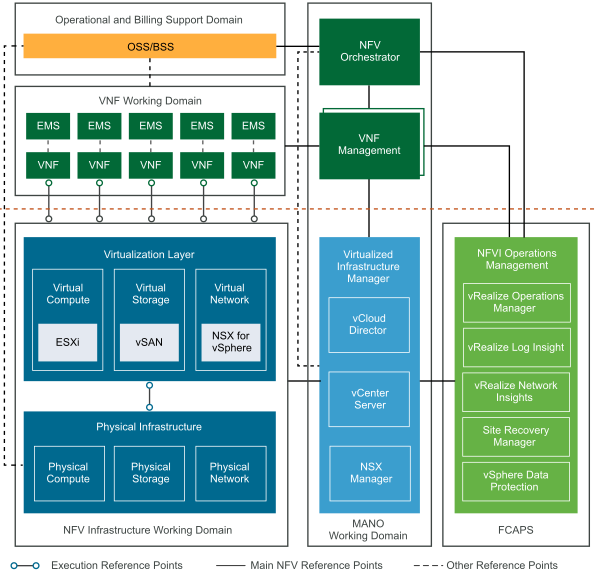
\includegraphics[width=0.7\textwidth]{graphics/vmware-nfv.png}
    \caption{Mapping dei prodotti VMware sull'architettura NFV \cite{vmware-vcloud}}
    \label{fig:vmware-nfv}
\end{figure}

% https://images.app.goo.gl/N55na3PmGGpkuGDd6
% \cite{vmware-vcloud} % https://images.app.goo.gl/3xsvPs54523TKozu9

% Ovviamente pure RedHat c'ha la sua, ne vogliamo parlare?
% https://images.app.goo.gl/gJxkHNwEEjgpzrx18
  \chapter{Sperimentazione}
\label{chap:lab}

% https://ntnuopen.ntnu.no/ntnu-xmlui/bitstream/handle/11250/2634012/no.ntnu:inspera:2440645.pdf

Dopo tante parole spese, è il momento giusto per soffermarsi a ricapitolare. Finora abbiamo visto le nozioni principali ed il percorso storico che hanno accompagnato lo sviluppo delle reti Internet, culminati nell'architettura ETSI NFV. Abbiamo parlato del software atto a realizzare un router interamente virtuale e delle ottimizzazioni necessarie affinché sia il più efficiente possibile, motivando ogni scelta. Infine, abbiamo accennato come questo software possa essere inserito in un più complesso sistema di orchestrazione, citando alcuni esempi.

Ora bisogna passare dalla teoria alla pratica. Questo capitolo tratta il nostro tentativo di deployare un router completamente virtuale sopra un hypervisor. In particolare, racconteremo le sfide, i problemi, le soluzioni e gli interrogativi ancora aperti. L'obiettivo è sperimentare quanto visto con VPP/DPDK e KVM, utilizzando TNSR come base di partenza. Non affronteremo il tema dell'orchestrazione e dell'automazione, scelta necessaria dato il tempo a disposizione.

\section{Hardware}

Conditio sine qua non per poter effettuare degli esperimenti è disporre di un laboratorio. La culla dove realizzarlo è stato il TOP-IX, l'Internet Exchange di Torino, che ha messo a disposizione hardware e conoscenze fondamentali. Nello specifico, abbiamo usato:

\begin{itemize}
    \item 2 server Supermicro SYS-1029U-TRTP2 (\textit{hyper1} e \textit{hyper2}) adibiti a virtualizzatori, ciascuno con a bordo 2 processori Intel Xeon Silver 4210R e 128 GB di RAM in configurazione a 3 canali. Inoltre, abbiamo montato le seguenti schede di rete aggiuntive:
    \begin{itemize}
        \item hyper1, Mellanox ConnectX-4 Lx CX4121A-XCAT con due interfacce a 10 Gbps
        \item hyper2, Intel X710-BM2 con due interfacce a 10 Gbps e Intel E810-CAM2 con due interfacce a 100 Gbps
    \end{itemize}
    \item 1 server Supermicro SYS-1029U-TRTP2 con 2 processori Intel Xeon Silver 4210R e 384 GB di RAM in configurazione a 3 canali, usato come traffic generator (\mbox{\textit{tg-monster}}), a cui è stata aggiunta una scheda Intel XXV710 con due interfacce a 25 Gbps
    \item 1 switch Nokia 7250 IXR-e Big 2QSFP28 8SFP28 24SFP+, centro stella della nostra rete
    \item 1 router Mikrotik CCR1036-8G-2S+ usato come traffic generator
    \item 1 switch Mikrotik CRS317-1G-16S+ usato come switch di supporto
\end{itemize}

Su tutti e tre i server abbiamo installato Ubuntu Server 20.04 LTS. Per hyper1 e hyper2 abbiamo aggiunto due parametri alla command line di Linux affinché il passthrough dei device PCIe avvenisse senza problemi:

\begin{figure}[h!]
\centering
\begin{BVerbatim}
GRUB_CMDLINE_LINUX_DEFAULT="intel_iommu=on iommu=pt"
\end{BVerbatim}
% \caption{C++ code}
\end{figure}

Quest'accortezza serve a istruire il sistema operativo su come inizializzare le \mbox{IOMMU}, l'equivalente delle MMU per i device PCI, permettendo ai dispositivi di accedere direttamente alla memoria (DMA) delle VM come se fossero bare metal.

Per la gestione delle macchine virtuali abbiamo usato \textit{virt-manager}, un front-end grafico di \textit{libvirt} che ha la funzione di interfacciarsi con svariati virtualization engines (tra cui KVM) ed astrarne il funzionamento.

A livello topologico ci sono due reti: la prima, quella di test, isolata dal resto, vede al centro lo switch Nokia con attorno collegati tutti i dispositivi. Sullo switch sono configurati due broadcast domain che raggruppano le interfacce: le porte pari in uno, le dispari nell'altro. 

Come da prassi consolidata, è poi presente una seconda rete, raccolta da un classico switch Ethernet, dedicata al management via SSH ed accessibile via VPN. In questa rete ciascuna VM dispone di un'interfaccia collegata ad un bridge virtuale connesso ad una porta fisica dedicata dell'hypervisor, il quale è a sua volta attestato sulla stessa rete in maniera indipendente tramite altre due porte LAN: su una è in ascolto il server SSH del sistema operativo, l'altra invece è gestita da IPMI, un management avanzato che permette di avere controllo dell'intero hardware da remoto.

\begin{figure}[htb]
    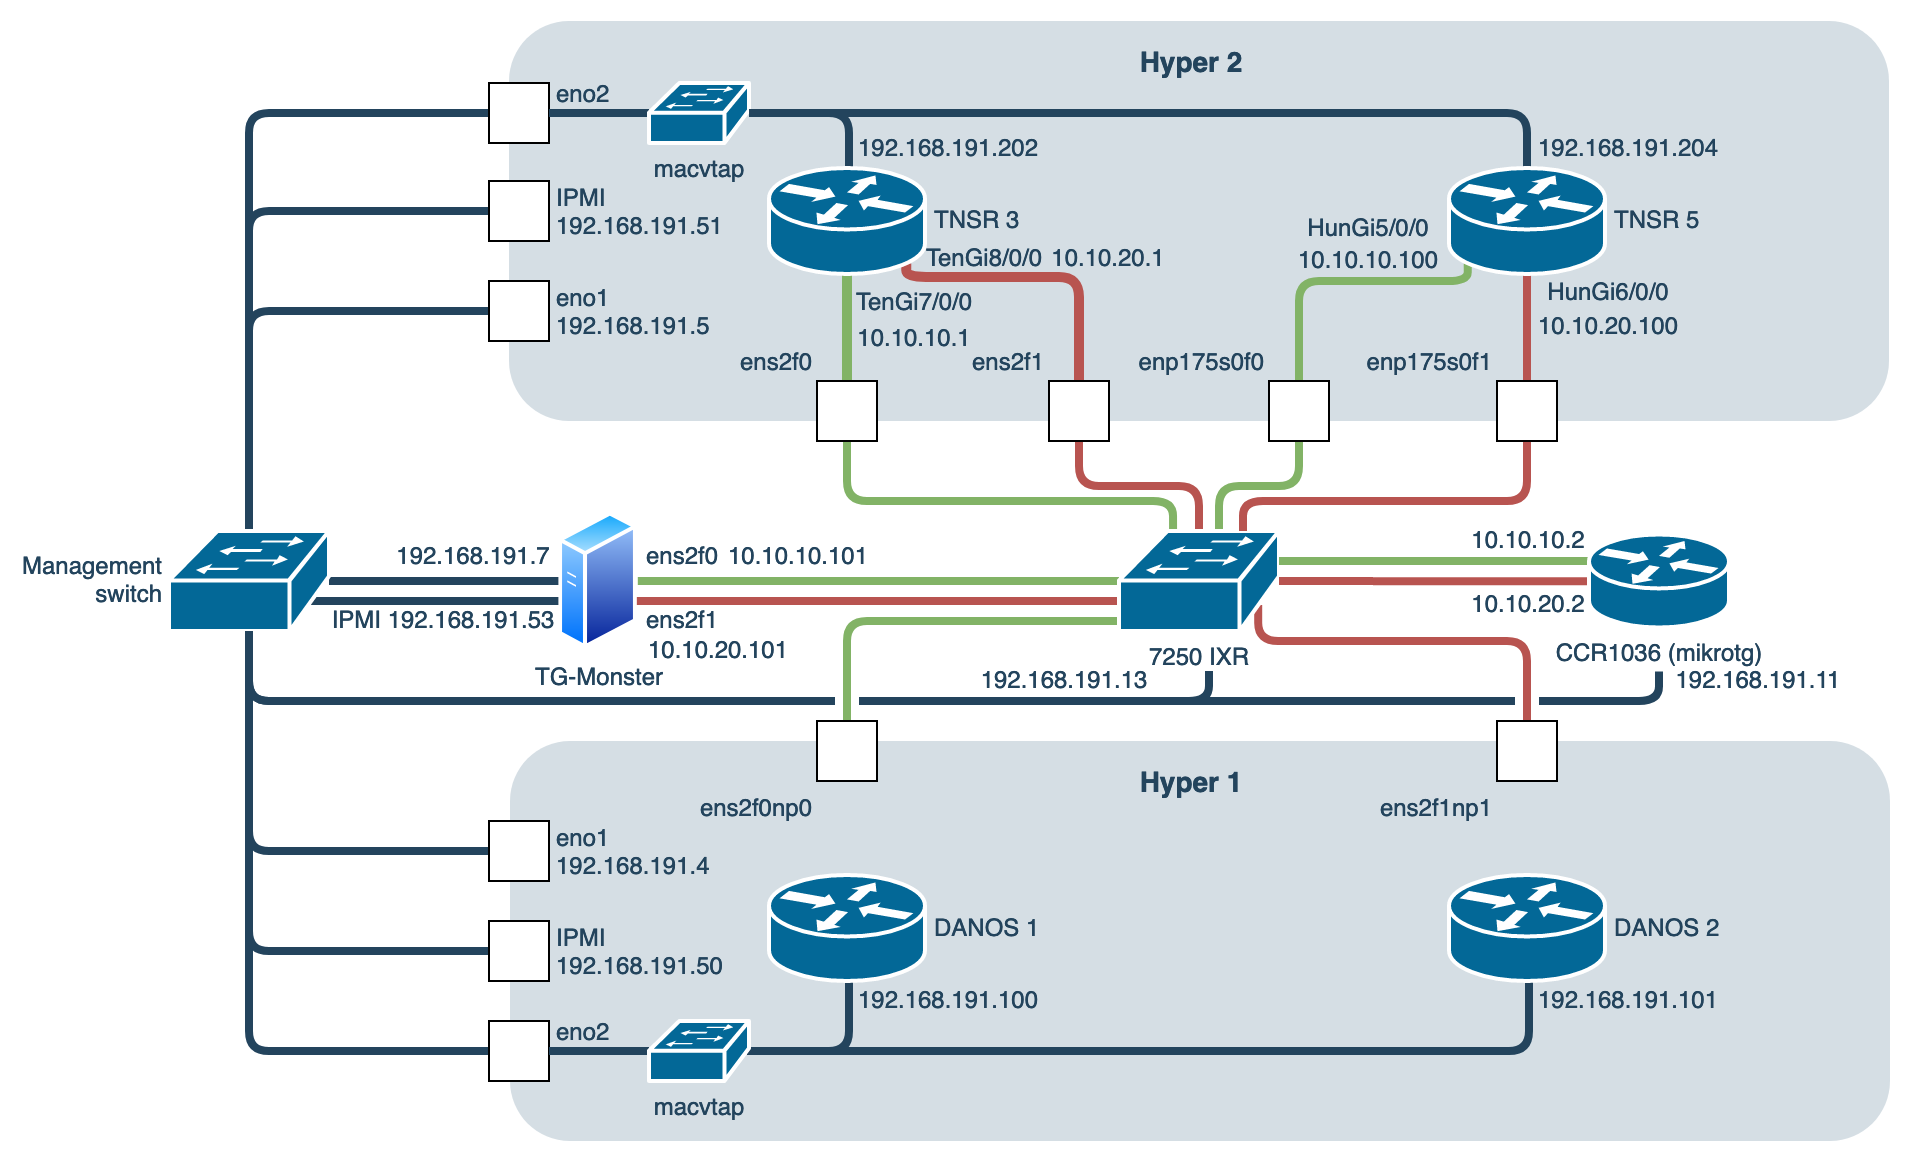
\includegraphics[width=0.8\textwidth]{graphics/vlan-191.png}
    \caption{Schema di rete del laboratorio}
    \label{fig:vlan-191}
\end{figure}

\section{Primi test}

Innanzitutto abbiamo provato a vedere se fosse possibile instaurare una sessione BGP tra pochi router, scambiandosi dei prefissi. La topologia base era costituita da tre router: R1 al centro, R2 ed R3 ai bordi, ciascuno su un sistema autonomo distinto. R1 simulava un route reflector e ridistribuiva i prefissi imparati via eBGP, R2 ed R3 possedevano ciascuno una LAN in classe C connessa e la annunciavano. Ogni router era identificato dall'indirizzo di loopback assegnato ad un'interfaccia dedicata. Le punto-a-punto erano realizzate semplicemente con un bridge virtuale nell'hypervisor.

\begin{figure}[htb]
    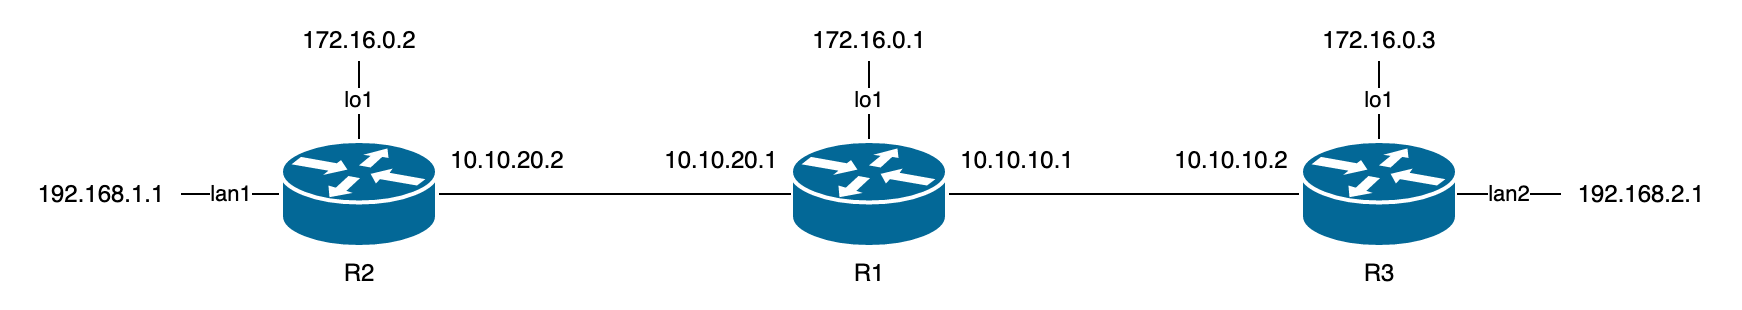
\includegraphics[width=0.8\textwidth]{graphics/bgp-topo-1.png}
    \caption{Topologia iniziale}
    \label{fig:bgp-topo-1}
\end{figure}

La rete funzionava ed era possibile contattare l'interfaccia \textit{lan2} di R3 dalla \textit{lan1} di R2, verificando nel traceroute che si passasse effettivamente per R1. Dapprima abbiamo usato TNSR su ciascun router, poi abbiamo provato a sostituirne alcuni con DANOS o VyOS, verificando il corretto funzionamento ogni volta. Ciò è stato utile per provare che non solo i diversi control plane funzionassero, ma che fosse anche possibile interconnettersi ad altri apparati tramite protocolli standard.

\section{SMT}

\textit{Simultaneous Multi-Threading} (SMT) è una tecnologia che consente a due o più thread applicativi di essere eseguiti contemporaneamente su uno stesso core fisico. Un moderno microprocessore dispone di abbondanti capacità di memorizzazione ed elaborazione, difficili da sfruttare appieno con il solo \textit{Instruction Level Parallelism} (ILP). Con SMT le risorse vengono partizionate dinamicamente e ripartite tra i thread con pochissimo overhead, poiché si può fare affidamento a tutto lo scheletro già presente per l'esecuzione multiple issue di ILP, apportando piccole modifiche.

Nel paragrafo \ref{sec:vpp} abbiamo visto come VPP sfrutti il processing vettoriale per aumentare il throughput, elaborando grandi insiemi di dati alla volta piuttosto che singolarmente. SMT d'altra parte, dividendo le risorse tra più thread, ottiene l'effetto contrario: ogni thread che operi a pieno regime potrà sfruttare solo metà delle \eng{instruction} cache e data cache disponibili nel core, intaccando sensibilmente le performance di VPP.

\begin{figure}[htb]
    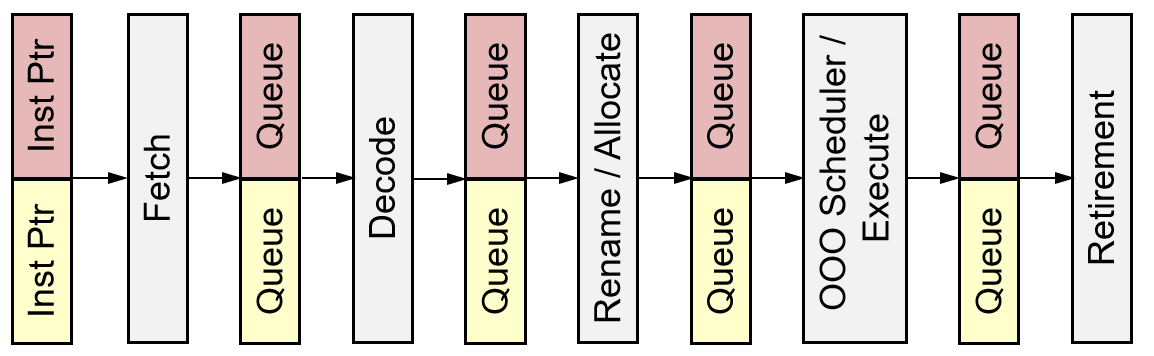
\includegraphics[width=0.7\textwidth]{graphics/smt.png}
    \caption{Ripartizione delle instruction queue in SMT}
    \label{fig:smt}
\end{figure}

Alcuni semplici test effettuati in locale hanno confermato quanto da molti riportato online: SMT, commercializzato da Intel col nome \textit{``Hyper-Threading''}, rallenta VPP, motivo per il quale abbiamo deciso di disabilitarlo fin da subito.

\section{Traffic generation}

% Appurato che il peering funzionasse, abbiamo staccato i due router laterali e mappato le porte di R1 sulle interfacce fisiche dell'hypervisor (PCI passthrough). Queste erano collegate al CRS317 al quale era connesso pure il CCR1036. Il Mikrotik, da specifica, è in grado di generare traffico a 10 Gbps verso destinazioni configurabili, adeguato al nostro obiettivo di raggiungere il \textit{line rate} escludendo dal test variabili legate al generatore.

A valle del controllo di configurazione BGP, abbiamo proceduto a verificare le prestazioni del singolo router. La macchina R1 ha visto le proprie interfacce mappate su quelle fisiche dell'hypervisor in PCI passthrough. A questo punto abbiamo utilizzato il router CCR1036 per generare diversi pattern di traffico passanti per R1. Il Mikrotik è stato scelto in quanto permette di generare flussi di 10 Gbps line rate su singola interfaccia in modalità stateless, valore adeguato al nostro obiettivo di test.

``Line rate'' è un termine che si riferisce alla capacità di un apparato di raggiungere e mantenere una certa velocità operativa indipendentemente dalla dimensione dei pacchetti dati. Come riferimento, si usa un pacchetto L2 da 64 byte (60 di payload + 4 di frame check sequence) a cui, nel caso di Ethernet, vanno aggiunti 8 byte di preambolo, 1 byte di epilogo e 11 byte di inter-frame gap, portando la dimensione totale a 84 byte. A questo punto è facile calcolare il packet-rate corrispondente a 10 Gbps:

\begin{equation} \label{eq:10g-line-rate}
    \frac{10\ Gbps}{84\ byte \cdot 8} \approx 14.88\ Mpps
\end{equation}

Il primo test ``a scatola chiusa'' ha mostrato che DANOS era in grado di raggiungere circa 11 Mpps nel puro forwarding IP tra due interfacce, mentre TNSR si fermava a metà: 5.5 Mpps. A questo punto le basi teoriche esposte nel \cref{chap:software} non erano ancora ben consolidate ed abbiamo cercato di indagare per scoprire la ragione di questi risultati, incuriositi dal fatto che uno fosse esattamente il doppio più veloce dell'altro.

\section{Receive Side Scaling}

Nessun microprocessore, per quanto potente, è in grado di scalare all'infinito accomodando moli sempre più crescenti di traffico. Occorre un metodo per suddividere il carico tra molteplici worker in maniera che possa essere gestito in parallelo. Il modo più intuitivo consisterebbe nel definire $n$ code in ricezione (\textit{receive queues} o \mbox{\textit{rx-queues}}) e ripartire i pacchetti tra esse secondo un algoritmo round-robin. Tuttavia un'equa spartizione di questo tipo avrebbe il probabile effetto di trattare diversamente pacchetti di uno stesso flusso end-to-end, generando imprevedibilità nella rete: i dati potrebbero giungere a destinazione seguendo strade diverse e con diverse latenze, andando direttamente a pesare su quei trasporti come TCP che devono riordinare i dati prima di consegnarli al livello applicativo, oppure perdersi in parte. Per questo motivo al round-robin tradizionale si preferisce una soluzione equivalente che cerchi di preservare ogni flusso nella sua interezza.

Receive Side Scaling (RSS) è l'approccio proposto da Microsoft e largamente adottato: un classificatore hardware ridistribuisce i pacchetti su un numero configurabile di code basandosi su un hash\footnote{\ Algoritmo proprietario calcolato dalla NIC stessa e diverso per ciascun produttore} degli indirizzi sorgente e destinazione di livello 3 e 4, oppure sulle etichette MPLS, assumendo così un significato semantico analogo alla flow label di IPv6.

\begin{figure}[htb]
    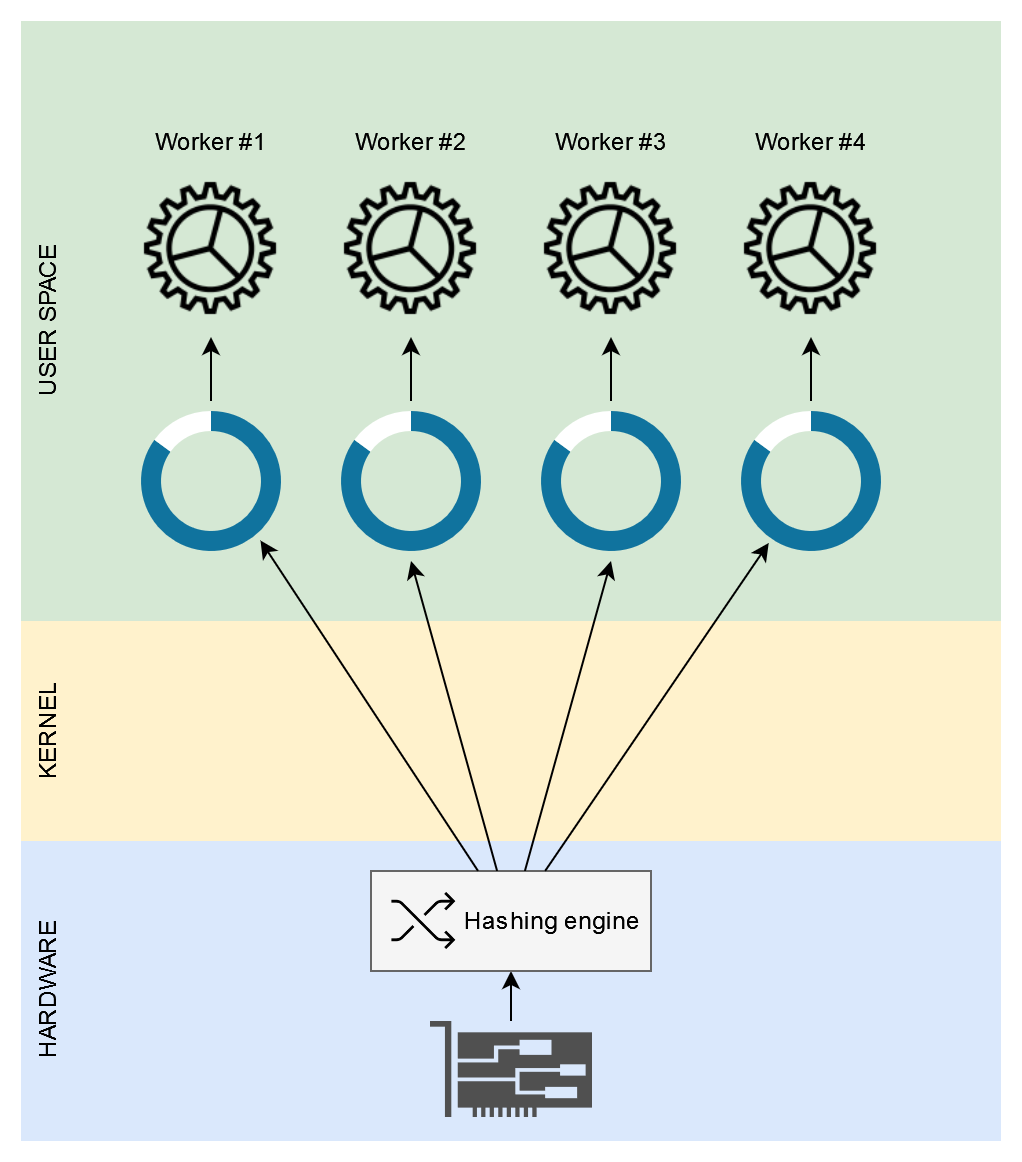
\includegraphics[width=0.7\textwidth]{graphics/rss.png}
    \caption{Receive Side Scaling\protect\footnotemark}
    \label{fig:rss}
\end{figure}
\footnotetext{\ I buffer sono rappresentati in user space, forma ottenibile con l'ausilio di DPDK}

Un criterio affine è adottato in ambiti diversi, come il load balancing: nel definire un \textit{link aggregation} (LAG) i vendor adottano un sistema simile per ripartire il traffico basandosi su hashing. Le NIC moderne, come la Intel E810 da noi testata, consentono di andare oltre e sostituire il classificatore con un microprogramma personalizzato. Questo apre ad un'infinità di possibilità come differenziare il traffico in base alla sua natura: un operatore mobile potrebbe voler dare priorità ai flussi LTE Voce a discapito dei pacchetti dati, assegnando ai primi delle code pregiate con worker dedicati e rilegando gli altri a buffer best effort con le risorse rimanenti.

Quanto appreso con RSS ci ha permesso di capire che DANOS stava adoperando dietro le quinte 2 rx-queues con altrettanti worker dedicati. TNSR invece di default ne usava una sola, ma a differenza di DANOS permetteva di modificare questo parametro. Alzando le rx-queues a 2 abbiamo ottenuto prestazioni in linea con DANOS. La vera sorpresa però è stata quando abbiamo ulteriormente aumentato fino a 4 code: i risultati erano identici. In seguito alla verifica inconcludente di molteplici configurazioni, abbiamo provato a replicare l'esperimento su hyper2 sfruttando la scheda Intel che fin da subito ha raggiunto il line rate.
% L'ipotesi più accreditata è che l'RSS della Mellanox non riuscisse a ripartire correttamente i flussi del Mikrotik su più code, essendo questi sostanzialmente identici end-to-end.
Pur non disponendo una prova formale, supponiamo che la funzione di hashing della modalità RSS implementata nella NIC Mellanox non riuscisse a ripartire correttamente su più code il traffico di test, probabilmente per mancanza di entropia negli \textit{headers} dei pacchetti utilizzati al fine del bilanciamento.
La Intel verosimilmente implementa un algoritmo di hashing diverso, in grado di distribuire equamente il traffico anche in casi come questo. Onde evitare il ripetersi dell'anomalia, si è deciso di cambiare traffic generator, installando TRex su \mbox{tg-monster} cosicché si potesse trarre vantaggio dalla maggiore entropia dei flussi.

\section{NUMA pinning} % isolcpus

Raggiunto il traguardo dei 10 Gbps line rate, lo step successivo era verificare quanto potesse scalare. Il CRS317 è stato sostituito dal Nokia, equipaggiato di porte a 25 e 100 Gbps, al posto del CCR1036 abbiamo messo il server dedicato con TRex e su hyper2 abbiamo montato la scheda Intel E810. Questa riorganizzazione era anche un buon momento per ottimizzare il layout fisico delle macchine virtuali: nel \cref{chap:virt} si è discusso di come un deploy NUMA-aware sia imprescindibile per raggiungere target di un certo calibro. A tal proposito, KVM permette di esplicitare i core fisici sui cui mappare i thread virtuali delle VM tramite l'attributo \verb|cpuset|.

\begin{figure}[htb]
    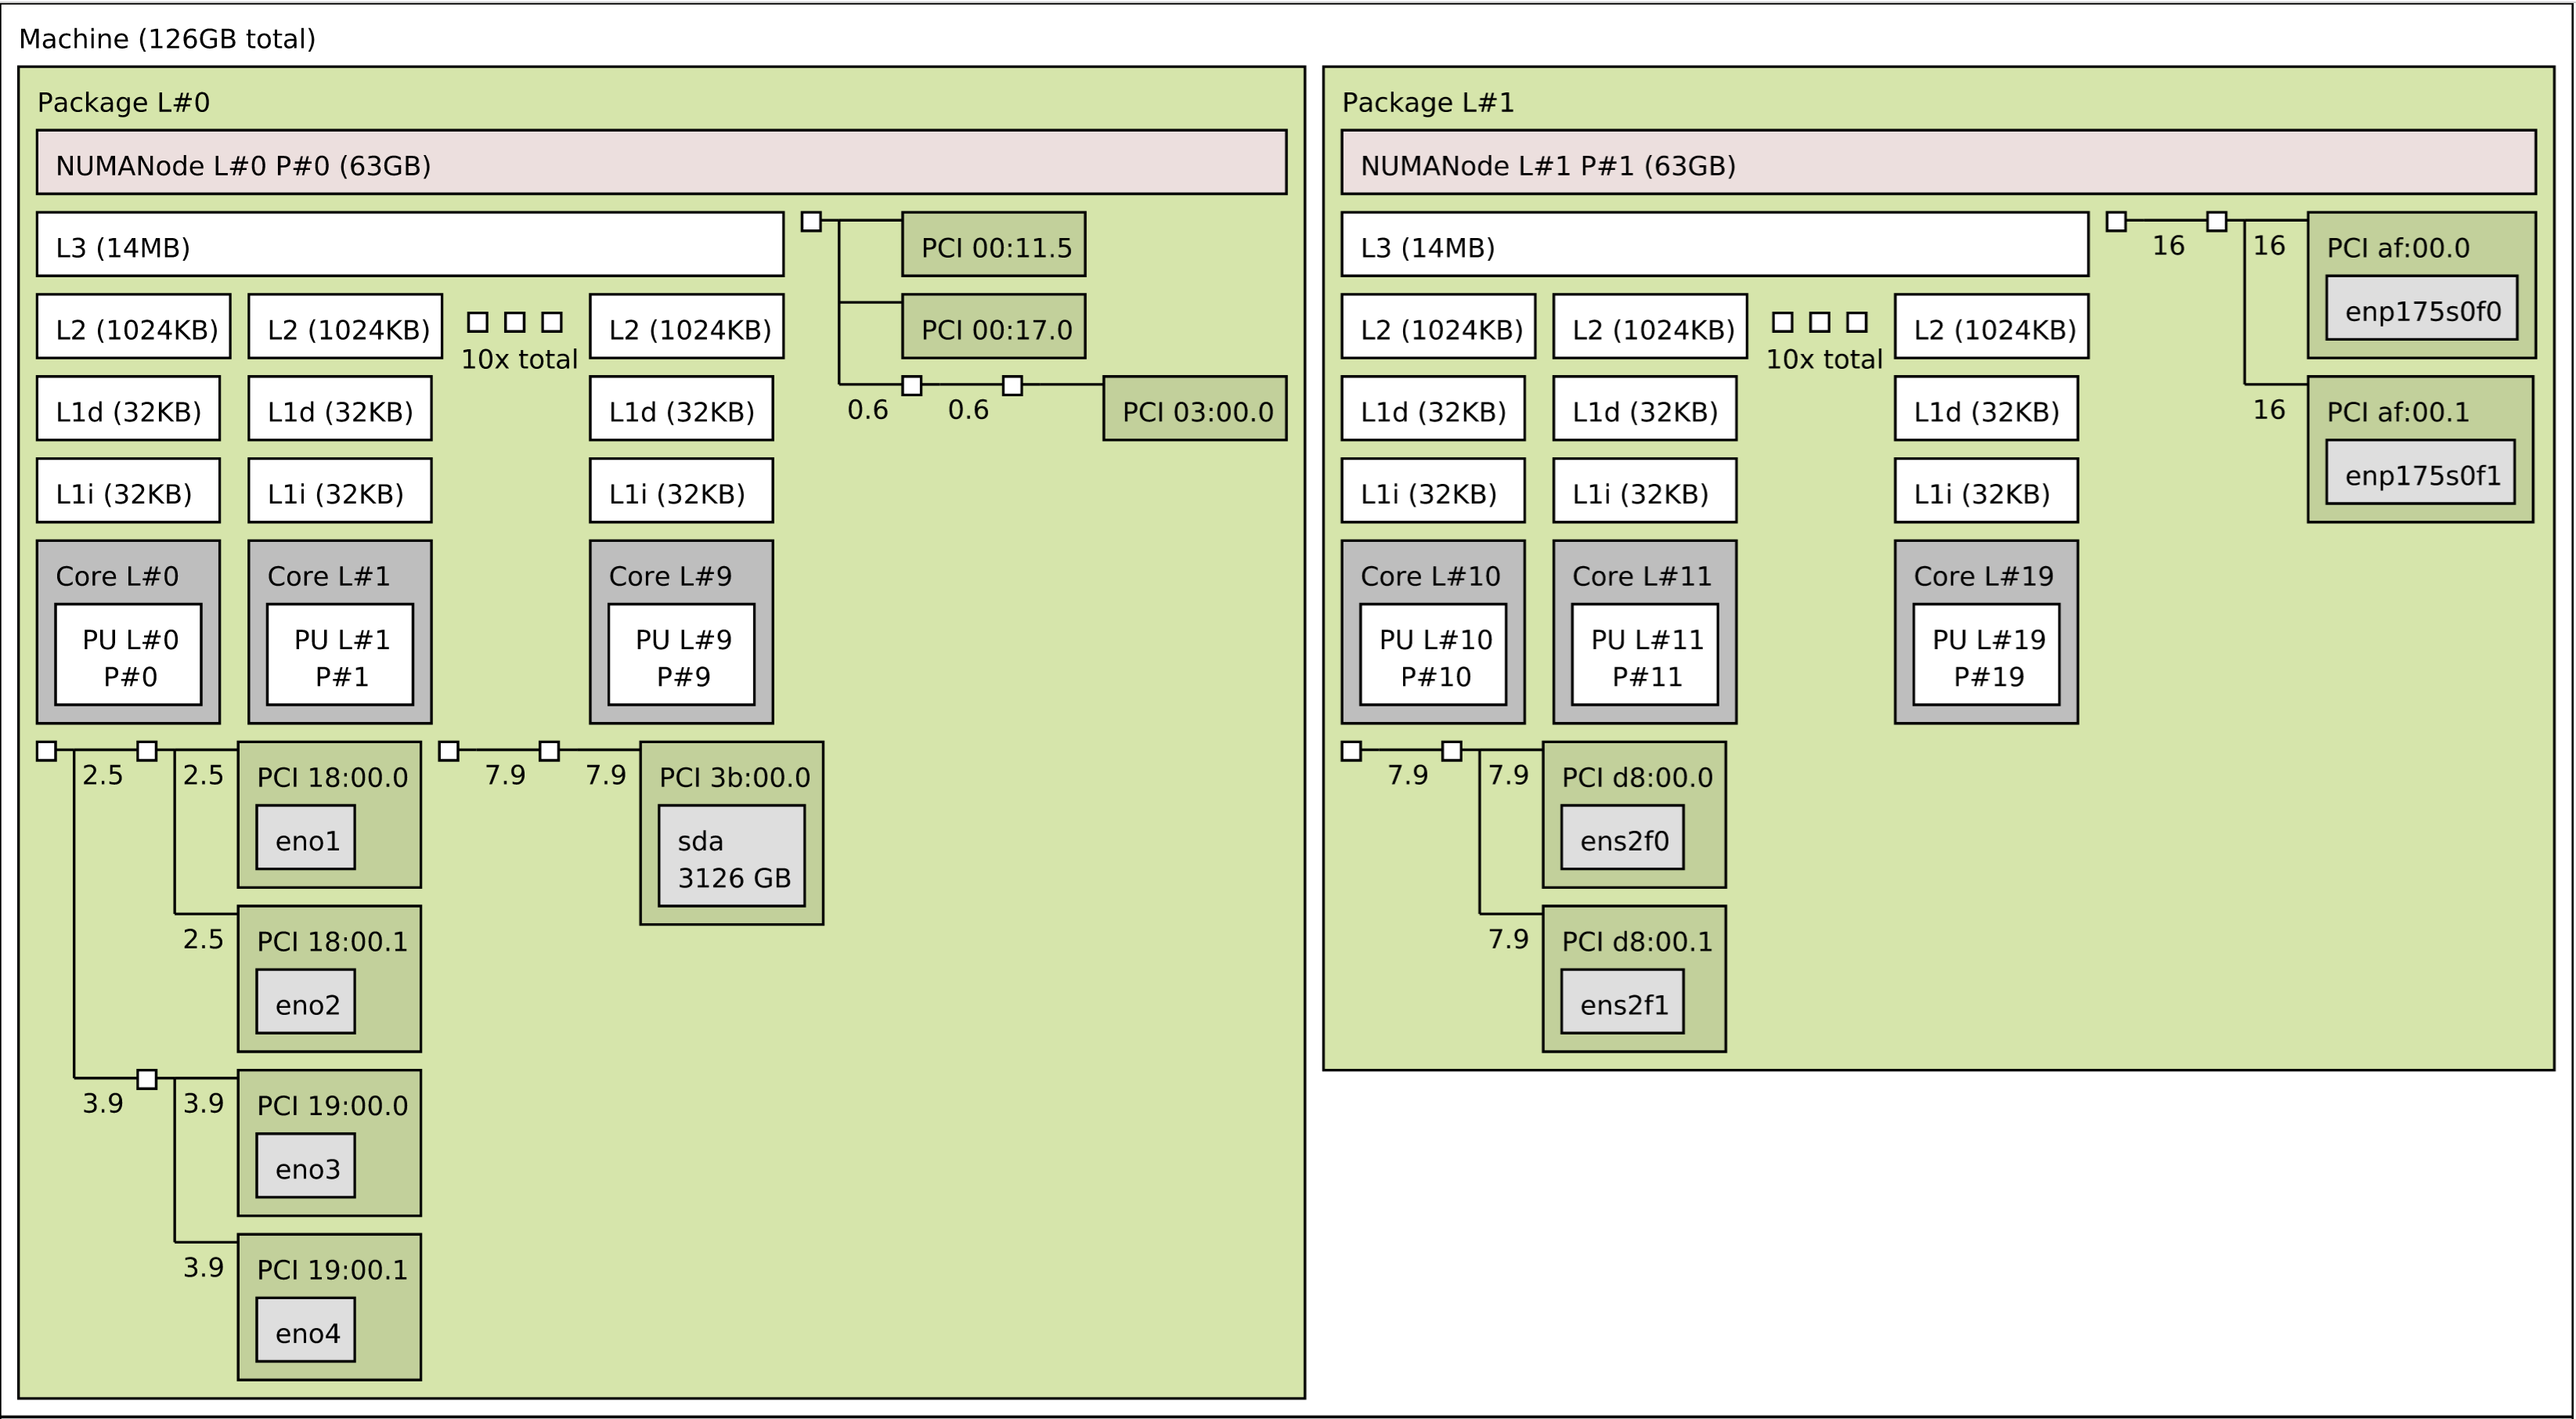
\includegraphics[width=0.8\textwidth]{graphics/hyper2topohd.png}
    \caption{Topologia fisica di hyper2}
    \label{fig:hyper2topo}
\end{figure}

In figura \ref{fig:hyper2topo} è rappresentata la topologia fisica di hyper2 ottenuta tramite lo strumento \verb|lstopo|. Si possono distinguere chiaramente i due nodi NUMA: del primo fanno parte \mbox{CPU0} (core da 0 a 9), \mbox{64 GB} di memoria, le 4 interfacce di rete integrate del server, lo storage (\textit{sda}) e altri dispositivi minori. Nel secondo invece troviamo CPU1 (core da 10 a 19), i restanti \mbox{64 GB} di RAM e le schede di rete aggiuntive: \textit{ens2} è la X710, mentre \textit{enp175s0} la E810; \textit{f0} ed \textit{f1} sono le due interfacce fisiche presenti su ciascuna NIC.

Per i test si è deciso di dedicare interamente CPU1 alla macchina virtuale con TNSR specificando l'attributo \verb|cpuset="10-19"| in KVM. Non solo, per evitare che quei core potessero essere usati dall'hypervisor per task di routine, li abbiamo esclusi dallo scheduling di Linux tramite il parametro \verb|isolcpus=10-19| alla cmdline del kernel. Così facendo la VM con TNSR ha assunto il controllo completo di CPU1 e dei device ad essa connessi, acquisiti con PCI passthrough. Volendo sarebbe stato possibile replicare una topologia NUMA verso la macchina virtuale, ma la poca familiarità con gli strumenti di virtualizzazione ci ha suggerito prudenza per non rischiare di compromettere i risultati sperimentali con errori grossolani dovuti all'inesperienza.

Il traffic generator prescelto, come anticipato, è stato TRex. Per il primo test abbiamo scelto un template IMIX da 1 Gbps, ossia un insieme di pacchetti di dimensione variabile rappresentativo di diverse tipologie di flussi dati: streaming, \eng{video conferencing}, navigazione web, mail, ecc. Il termine IMIX è infatti una sincrasi di ``Internet Mix'' per indicare la natura del traffico.

\begin{figure}[h!]
\centering
\begin{BVerbatim}
./t-rex-64 -f avl/sfr_delay_10_1g.yaml -m 25 -c 4 -l 1000
\end{BVerbatim}
% \caption{C++ code}
\end{figure}

Con questo comando abbiamo istruito TRex affinché generasse 25 Gbps di \eng{throughput} aggregato\footnote{\ Bidirezionale, circa 20 Gbps in una direzione e 5 Gbps nell'altra}: a partire da una base di 1 Gbps, questa andava amplificata 25 volte ed il test eseguito utilizzando 4 core del server.

\begin{figure}[htb]
    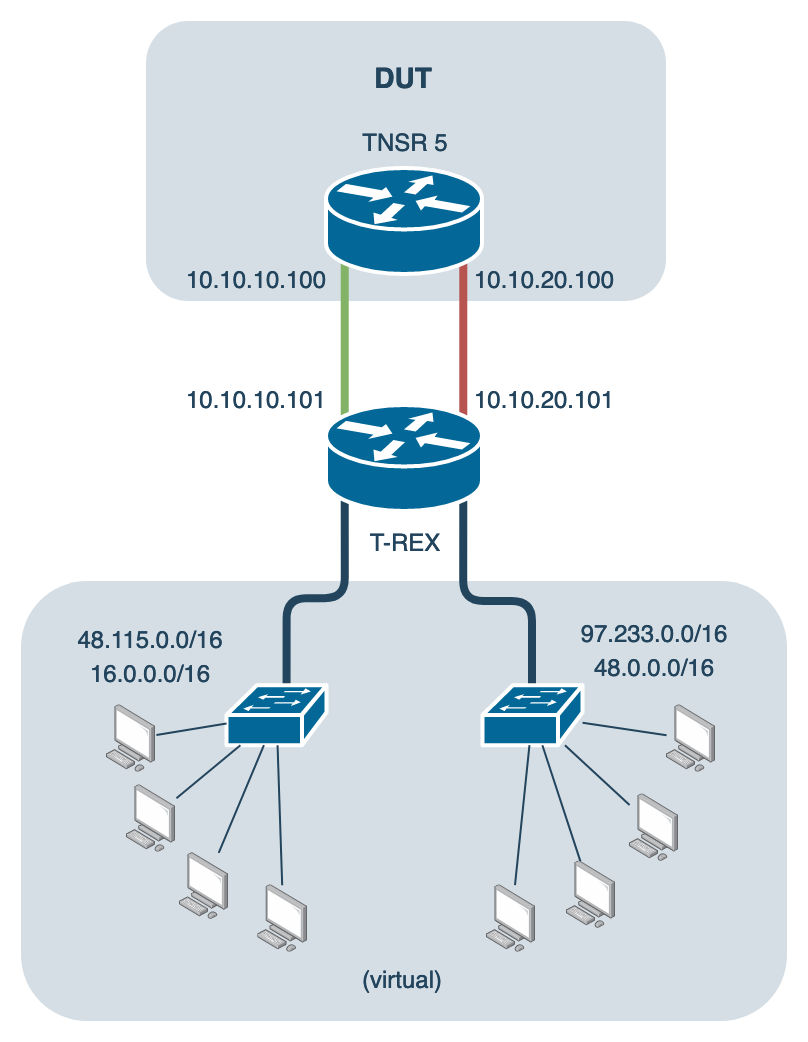
\includegraphics[width=0.5\textwidth]{graphics/trex-tnsr-dut.png}
    \caption{Schema del test}
    \label{fig:trex-tnsr-dut}
\end{figure}

I primi risultati sono stati soddisfacenti: 25 Gbps di traffico IMIX corrispondono ad appena 5.35 Mpps, entro il limite determinato sperimentalmente di un singolo core del nostro virtualizzatore. Quando però abbiamo provato ad aumentare il numero di worker per ripartire il carico, il router ha letteralmente smesso di funzionare: la quasi totalità dei pacchetti andava perduta o subiva latenze migliaia di volte più grandi di quelle misurate in precedenza. Dopo svariati tentativi andati a vuoto, non siamo riusciti a determinare la causa di questo problema, ma possiamo formulare delle ipotesi:

\begin{enumerate}
    \item TNSR viene fornito con la penultima versione di VPP e DPDK attualmente disponibili e noi, seguendo le indicazioni del manuale stesso di DPDK, abbiamo installato la penultima versione di driver e firware della scheda di rete. La prima ipotesi è dunque che si tratti di un bug, ma per verificarla occorrerebbe configurare da zero un'installazione di Linux con le ultime versioni di kernel, driver, VPP/DPDK e FRR.
    \item Tra le ottimizzazioni non prese in considerazione vi sono quelle legate alla memoria. In primis non abbiamo verificato che tutta la memoria riservata per la macchina virtuale risiedesse nel nodo NUMA in cui questa era collocata, fattore che però non avrebbe potuto a nostro avviso compromettere così gravemente le performance. In secondo luogo c'è il discorso \textit{hugepages}: come accennato nel paragrafo \ref{sec:dpdk}, DPDK fa uso di grandi aree di memoria contigua su cui mappare i buffer delle schede di rete. Linux permette di utilizzare 3 diverse dimensioni per le pagine di memoria: 4 KB (default), 2 MB e 1 GB, queste ultime definite ``huge pages''. Di default con KVM non è disponibile il supporto a pagine da 1 GB all'interno della VM: non sappiamo cosa succederebbe se il sistema operativo ospite provasse ugualmente ad allocarne, ma presumibilmente nulla di buono.
\end{enumerate}

La seconda ipotesi potrebbe essere avallata da un altro problema verificatosi in più occasioni: ogni volta che cercavamo di cambiare al volo il numero di code utilizzate dalla scheda di rete era necessario riavviare sia la macchina virtuale che l'hypervisor affinché queste modifiche avessero effetto. Questo comportamento è insolito e a riguardo possono esserci due spiegazioni:

\begin{enumerate}
    \item Riavviare il dispositivo, reinizializzandolo, provvede al reseeding dell'hashing engine di RSS che ha il compito di canalizzare il traffico sulle \mbox{rx-queues}. La nostra congettura è che questo non venga correttamente resettato quando si cambia dinamicamente il numero di code.
    \item Anche in questo caso il mapping tra memoria della macchina virtuale, memoria fisica e IOMMU potrebbe essere venuto meno, portando la NIC a scrivere i pacchetti ricevuti in aree di memoria non corrispondenti alle code allocate da DPDK.
\end{enumerate}

Tutti questi scenari sono difficili da investigare poiché richiedono grande dimestichezza con gli strumenti di diagnostica e una profonda conoscenza del funzionamento interno del software sottostante. Un aiuto potrebbe venire dall'indagare separatamente i problemi software da quelli legati all'infrastruttura di virtualizzazione, installando TNSR (o chi per esso) direttamente sul server fisico. Lo scopo di questa tesi però era indagare entrambi gli aspetti, motivo per il quale si era deciso di intraprendere la strada della virtualizzazione fin dall'inizio.

Purtroppo il tempo da dedicare a questa esperienza è terminato e gli interrogativi sopra esposti rimarranno aperti fino a quando qualcuno non si cimenterà nuovamente nell'impresa. Ammetto che non mi dispiacerebbe riprendere in mano questi argomenti un giorno, vedremo cosa ci riserverà il futuro.



% NUMA images
% https://cloudarchitectmusings.com/2012/12/17/the-impact-of-numa-on-virtualizing-business-critical-applications/
% https://frankdenneman.nl/2010/09/13/esx-4-1-numa-scheduling/ <<<===== CTO WMware
  \chapter{Conclusioni}
\label{chap:conclusioni}

Volgendosi all'indietro, come per scorgere i propri passi, la strada percorsa è lunga. Tutto è iniziato dall'idea di poter interconnettere reti all'edge, complice anche il repentino aumento del traffico nazionale dovuto alla pandemia, riscoprendo il vecchio detto \textit{\eng{``keep the local traffic local''}}. La vera sfida però era riuscirvi con un'infrastruttura completamente virtuale. Questo ha significato dover approfondire framework prima sconosciuti come VPP e DPDK, nonché studiare i meccanismi di virtualizzazione ed il funzionamento del kernel Linux che oggi sono alla base del mondo cloud. L'esperienza è culminata con una prova sul campo di quanto appreso, da cui sono emerse nuove problematiche e nuove conoscenze. Sono grato ai miei relatori per avermi sostenuto e guidato in questo cammino lungo e colmo di soddisfazioni.

\section{Sviluppi futuri}

Di tutte le funzioni che si possono virtualizzare, il puro routing è forse una delle meno sensate: al crescere del traffico, oltre qualche decina di Gigabit al secondo, diventa economicamente sconveniente -- sia in termini di costo capitale che di costo energetico per traffico trasferito -- affidarsi a soluzioni interamente virtuali. Inoltre, l'elevata preparazione richiesta in termini di forza lavoro è difficile da reperire sul mercato. A chi, nonostante ciò, volesse dedicarvisi, magari per interesse accademico o più semplice anticonformismo, consiglio di sfruttare quanto descritto in queste pagine per ripartire dal basso: cominciare da un sistema operativo nudo sul quale avere maggiore controllo delle diverse componenti software, magari basandosi su qualche distribuzione ``rolling'' di Linux. TNSR si è rivelato un buon prodotto con cui iniziare, ma al crescere delle difficoltà il funzionamento interno è difficile da indagare senza supporto commerciale. Un altro consiglio è quello di consultare i manuali Red Hat riguardo a KVM: sono molto curati e trattano in maniera approfondita tutti i temi legati alla virtualizzazione. Altra fonte importante è il blog di Pim van Pelt, vera miniera di informazioni.

Vi è poi tutta la classe di ottimizzazioni legate all'utilizzo dei canali di memoria per trasferire parallelamente pacchetti senza che questi si accavallino tra banchi diversi, sprecando banda: a fianco dell'analisi teorica è fondamentale affinare il setup pratico in funzione della piattaforma hardware usata. I manuali di DPDK coprono questi temi in maniera esaustiva.
% purtroppo non ho avuto tempo di vedere questi temi con la dovuta attenzione, ma i manuali di DPDK li coprono in maniera esaustiva.

% Infine, dopo aver padroneggiato l'architettura virtuale, ci si può cimentare con l'orchestrazione vera e propria, l'automazione e la necessaria manutenzione di un'infrastruttura operativa in produzione. Io mi fermo qui, sperando di aver stuzzicato il vostro interesse e la passione che ci accomuna.

Infine, con un'infrastruttura virtuale di grandi dimensioni diventa imprescindibile adottare un sistema di orchestrazione e automazione: su questo punto l'esperienza maturata a livello industriale e non è sufficientemente ampia, essendo la virtualizzazione un approccio standard da ormai molti anni.

Io mi fermo qui, sperando di aver stuzzicato il vostro interesse e la passione che ci accomuna.
  
  % Leave an empty line here or LaTeX will complain
\end{mainmatter}

%% Produce the appendices
\begin{appendices}
  \chapter{Configurazioni}
\label{chap:config}

\section{10 Gbps line rate}

\begin{lstlisting}
configuration history enable

nacm disable
nacm read-default deny
nacm write-default deny
nacm exec-default deny
nacm group admin
    member root
    member tnsr
exit
nacm rule-list admin-rules
    group admin
    rule permit-all
        module *
        access-operations *
        action permit
    exit
exit
nacm enable

dataplane cpu workers 4
dataplane ethernet default-mtu 9000
dataplane dpdk dev 0000:07:00.0 network num-rx-queues 4
dataplane dpdk uio-driver igb_uio
dataplane buffers buffers-per-numa 32768
dataplane statseg heap-size 96M


nat global-options nat44 max-translations-per-thread 128000
nat global-options nat44 enabled false

interface TenGigabitEthernet7/0/0
    enable
    ip address 10.10.10.1/24
exit
interface TenGigabitEthernet8/0/0
    enable
    ip address 10.10.20.1/24
exit

nat ipfix logging domain 1
nat ipfix logging src-port 4739
nat nat64 map parameters
    security-check enable
exit

interface TenGigabitEthernet7/0/0
exit
interface TenGigabitEthernet8/0/0
exit

route dynamic manager
exit

route dynamic ospf6
exit

route dynamic bgp
    disable
exit

route dynamic ospf
exit

route dynamic rip
exit

dhcp4 server
    lease persist true
    lease lfc-interval 3600
    interface socket raw
exit

unbound server
    enable ip4
    enable tcp
    enable udp
    enable harden glue
    enable hide identity
    port outgoing range 4096
exit

snmp host disable
\end{lstlisting}

\section{25 Gbps IMIX}

\begin{lstlisting}
configuration history enable

nacm disable
nacm read-default deny
nacm write-default deny
nacm exec-default deny
nacm group admin
    member root
    member tnsr
exit
nacm rule-list admin-rules
    group admin
    rule permit-all
        module *
        access-operations *
        action permit
    exit
exit
nacm enable

dataplane ethernet default-mtu 1500
dataplane dpdk dev 0000:05:00.0 network num-rx-queues 2
dataplane dpdk dev 0000:05:00.0 network num-tx-queues 2
dataplane dpdk dev 0000:06:00.0 network num-rx-queues 2
dataplane dpdk dev 0000:06:00.0 network num-tx-queues 2
dataplane dpdk uio-driver igb_uio
dataplane buffers buffers-per-numa 32768
dataplane statseg heap-size 96M


nat global-options nat44 max-translations-per-thread 128000
nat global-options nat44 enabled false

route table ipv4-VRF:0
    id 0
exit


interface HundredGigabitEthernet5/0/0
    enable
    ip address 10.10.10.100/24
exit
interface HundredGigabitEthernet6/0/0
    enable
    ip address 10.10.20.100/24
exit

nat ipfix logging domain 1
nat ipfix logging src-port 4739
nat nat64 map parameters
    security-check enable
exit

route table ipv4-VRF:0
    id 0
    route 16.0.0.0/16
        next-hop 5 via 10.10.10.101
    exit
    route 48.0.0.0/16
        next-hop 6 via 10.10.20.101
    exit
    route 48.115.0.0/16
        next-hop 1 via 10.10.10.101
    exit
    route 97.233.0.0/16
        next-hop 2 via 10.10.20.101
    exit
exit


interface HundredGigabitEthernet5/0/0
exit
interface HundredGigabitEthernet6/0/0
exit

route dynamic manager
exit

route dynamic ospf6
exit

route dynamic bgp
    disable
exit

route dynamic ospf
exit

route dynamic rip
exit

dhcp4 server
    lease persist true
    lease lfc-interval 3600
    interface socket raw
exit

unbound server
    enable ip4
    enable tcp
    enable udp
    enable harden glue
    enable hide identity
    port outgoing range 4096
exit

snmp host disable
\end{lstlisting}

\section{TRex 25 Gbps IMIX}

\begin{lstlisting}
-Per port stats table 
      ports |               0 |               1 
 -----------------------------------------------------------------------------------------
   opackets |      7171065817 |      9308315110 
     obytes |   2273140861735 |   7338223064797 
   ipackets |      9176666445 |      7110502048 
     ibytes |   7236145304759 |   2253798106905 
    ierrors |               0 |               0 
    oerrors |               0 |               0 
      Tx Bw |       5.94 Gbps |      19.16 Gbps 

-Global stats enabled 
 Cpu Utilization : 41.8  %  30.0 Gb/core 
 Platform_factor : 1.0  
 Total-Tx        :      25.11 Gbps  
 Total-Rx        :      24.86 Gbps  
 Total-PPS       :       5.38 Mpps  
 Total-CPS       :     103.07 Kcps  

 Expected-PPS    :       5.38 Mpps  
 Expected-CPS    :     103.07 Kcps  
 Expected-BPS    :      25.10 Gbps  

 Active-flows    :   106534  Clients :      511   Socket-util : 0.3869 %    
 Open-flows      : 316342112  Servers :     5621   Socket :   124524 Socket/Clients :  243.7 
 drop-rate       :       0.00  bps   
 current time    : 3070.7 sec  
 test duration   : 529.3 sec  

-Latency stats enabled 
 Cpu Utilization : 0.1 %  
 if|   tx_ok , rx_ok  , rx check ,error,       latency (usec) ,    Jitter          max window 
   |         ,        ,          ,     ,   average   ,   max  ,    (usec)                     
 ---------------------------------------------------------------------------------------------------------------- 
 0 |  3069370, 2989709,         0,26437,         30  ,  120142,       8      |  74  934  57  60  83  74  62  199  5856  156  56  173  70 
 1 |  3069370, 3036630,         0, 6373,         39  ,  120260,       4      |  37  960  785  575  559  8140  7660  764  5804  889  5658  184  5874
\end{lstlisting}
\end{appendices}

%% Produce the un-numbered back matter (e.g. colophon,
%% bibliography, tables of figures etc., index...)
\begin{backmatter}
  %% You're recommended to use the eprint-aware biblio styles which
%% can be obtained from e.g. www.arxiv.org. The file mythesis.bib
%% is derived from the source using the SPIRES Bibtex service.
%\bibliographystyle{h-physrev}
%\bibliography{mythesis}
%\bibliographystyle{unsrt}
%\bibliography{bibliography}
\printbibliography[heading=bibintoc]

%% I prefer to put these tables here rather than making the
%% front matter seemingly interminable. No-one cares, anyway!
% \listoffigures
% \listoftables

%% If you have time and interest to generate a (decent) index,
%% then you've clearly spent more time on the write-up than the 
%% research ;-)
%\printindex

\end{backmatter}

%% Close
\end{document}
